\begin{summary}
First, new picking/weighting methods developed here and previously published
picking/weighting methods are compiled together to generate 168 different
paleomagnetic APWPs. Then, the APWP similarity measuring tool is used to find
which method\(s\) is$(are)$ good or bad.
\end{summary}

\begin{keywords}
  Moving Average \textendash{} Weighting \textendash{} APWP \textendash{}
  Paleomagnetism.
\end{keywords}

\section{Introduction}

APWPs are generated by combining paleomagnetic poles for a particular rigid
block over the desired age range to produce a smoothed path. See the
Supplementary Material for some examples how the pole datasets are constrained
first.

\subsection{Not All Data Are Created Equal}

However, uncertainties in the age and location of paleomagnetic poles can vary
greatly for different poles.

\subsubsection{Age Error}

Although remanent magnetizations are generally assumed to be primary, many
events can cause remagnetisation (in which case the derived pole is `younger'
than the rock). If an event that has occurred since the rock's formation that
should affect the magnetisation (e.g., folding, thermal overprinting due to
intrusion) can be shown to have affected it, then it constrains the
magnetisation to have been acquired before that event. Recognising or ruling
out remagnetisations depends on these field tests, which are not always
performed or possible. Even a passed field test may not be useful if field test
shows magnetisation acquired prior to a folding event tens of millions of years
after initial rock formation.

The most obvious characteristic we can observe from paleomagnetic data is that
some poles have very large age ranges, e.g., more than 100 Myr. The
magnetization age should be some time between the information of the rock and
folding events. There are also others where we have similar position but the age
constraint is much narrower, e.g. 10 Myr window or less. Obviously the latter
kind of data is more valuable than the one with large age range.

\subsubsection{Position Error}

The errors of pole latitudes and longitudes are 95\% confidence ellipses, which
also vary greatly in magnitude. All paleomagnetic poles have some associated
uncertainties due to measurement error and the nature of the geomagnetic field.
More uncertainties can be added by too few samples, sampling spanning too short
a time range to approximate a GAD field, failure to remove overprints during
demagnetisation, etc.

\subsubsection{Data Consistency}

Paleomagnetic poles of a rigid plate or block should be continuous time series.
For a rigid plate, two poles with similar ages shouldn't be dramatically
different in location. Sometimes, this is the case. Sometimes we have further
separated poles with close ages.

There are a number of possible causes for these outliers, including:

\verb"Lithology"

For poor consistency of data, it is potentially because of different
inclinations or declinations. The first thing we should consider about is their
lithology. We want to check if the sample rock are igneous or sedimentary,
because sediment compaction can result in anomalously shallow
inclinations~\cite{T18}. In addition, we also can check if the rock are redbeds
or non-redbeds. Although whether redbeds record a detrital signal or a later
Chemical Remanent Magnetization (CRM) is still somewhat controversial, both
sedimentary rocks and redbeds could lead to inconsistency in direction compared
to igneous rocks.

\verb"Local Rotations"

Local deformation between two paleomagnetic localities invalidates the rigid
plate assumption and could lead to inconsistent VGP directions. So if
discordance is due to local deformation, and we would ideally want to exclude
such poles from our APWP calculation.

\verb"Other Factors"

In most cases, mean pole age (centre of age error) has just been binned. If
any of the poles have large age errors, they could be different ages from each
other and sample entirely different parts of the APWP\@. Conversely, if any of
the poles have too few samples, or were not sampled over enough time to average
to a GAD field, a discordant pole may be due to unreduced secular variation.

\subsubsection{Data Density}

As we go back in time, we have lower quality and lower density (or quantity) of
data, for example, the Precambrian or Early Paleozoic paleomagnetic data are
relatively fewer than Middle-Late Phanerozoic ones, and most of them are not
high-quality, e.g., larger errors in both age and location. The combination of
lower data quality with lower data density means that a single `bad' pole (with
large errors in age and/or location) can much more easily distort the
reconstructed APWP, because there are few or no `good' poles to counteract its
influence.

Data density also varies between different plates. E.g., we have a relatively
high density of paleomagnetic data for North American Craton (NAC), but few
poles exist for Greenland and Arabia. Based on mean age (mean of lower and upper
magnetic ages), for 120\textendash0 Ma, the \textbf{Global Paleomagnetic
Database} (GPMDB) version 4.6b~\cite{P05} has more than 130 poles for NAC, but
only 17 for Greenland and 24 for Arabia.

\subsubsection{Publication Year}

The time when the data was published should also be considered, because
magnetism measuring methodology, technology and equipments have been improved
since the early 20th century. For example, stepwise demagnetisation, which is
the most reliable method of detecting and removing secondary overprints, has
only been in common use since the mid 1980s.

In summary, not all paleomagnetic poles are created equal, which leads to an
important question: how to best combine poles of varying quality into a coherent
and accurate APWP\@?

\subsection{Existing Solutions and General Issues}

Paleomagnetists have proposed a variety of methods to filter so-called ``bad''
data, or give lower weights to those ``bad'' data before generating an APWP,
e.g., two widely used methods: the V90 reliability criteria~\cite{v90} and the
BC02 selection criteria provided by Besse \& Courtillot \shortcite{B02}.
Briefly, the V90 criteria for paleomagnetic results includes seven criteria: (1)
Well determined age; (2) At least 25 samples with Fisher~\cite{F53} precision
$\kappa$ greater than 10 and $\alpha95$ less than 16\degree; (3) Detailed
demagnetisation results reported; (4) Passed field tests; (5) Tectonic coherence
with continent and good structural control; (6) Identified antipodal reversals;
(7) Lack of similarity with younger poles~\cite{T92}. The total criteria
satisfied (0\textendash7) is then used as a measure of a paleomagnetic result's
overall reliability, which is known as Q (quality) factor~\cite{T92}. Q factor
is indeed a very straightforward way to get a quantitalized reliability score.
Also it then can be conveniently used in the later calculations of
APWPs~\cite{T92}. But at the same time this is a fairly basic filter that lumps
together criteria that may not be equally important. Compared with V90, the BC02
criteria suggests stricter filtering, e.g., using only poles with at least 6
sampling sites and 36 samples, each site having $\alpha95$ less than 10\degree\
in the Cenozoic and 15\degree\ in the Mesozoic. B02 is also straightforward and
convenient to use, but some useful data may be filtered out and wasted
especially for a period where there are only limited number of data. In
addition, there has been limited study of how effective these marking/filtering
methods are at reconstructing a `true' APWP, and for most studies after a basic
filtering of `low quality' poles, the remaining poles are, in fact, treated
equally.

Above all, there haven't been any real attempts to study how APWP fits may be
improved by filtering/weighting data. This paper is presented to address these
issues.


\section{Methods}

For most of Earth history, concretely for times before c. 170 Ma, the age of the
oldest magnetic anomaly identification, paleomagnetism is the only accepted
quantitative method for reconstructing plate motions and past paleogeographies.
After about 170 Ma, multiple data sources can help constrain plate motions in
more accurate ways. One of the most developed and studied plate kinematics
models is the Fixed Hotspot Model (FHM)~\cite{M93,M99}, which assumes the
Atlantic and Indian hotspots are relatively fixed. Another one is the Moving
Hotspot Model (MHM)~\cite{O05}, which is based on mantle convection models that
indicate large motions of the Indo-Atlantic hotspots. Such a model like FHM or
MHM can predict APWPs for main continents, e.g.\ the North America (Plate ID
101) (Fig.~\ref{fig-fhsPred} and Fig.~\ref{fig-mhsPred}), the India (501)
(Fig.~\ref{fig-fhsPred501} and Fig.~\ref{fig-mhsPred501}) and the Australia
(801) (Fig.~\ref{fig-fhsPred801} and Fig.~\ref{fig-mhsPred801}). For about 120
Ma to the present, India drifts much faster than North America and Australia.
North America has been drifting rather slow. Australia's drifting rate is
between them. In addition, India drifts almost north, whereas North America
east and then north, and Australia west and then north. So these three
continents are representatives for three different types of plate kinematics.

\subsection{Reference Path: The Hotspot Model Predicted}

The oldest pole that can be predicted from the FHM is about 120 Ma. The North
American 120\textendash0 Ma APWP predicted from this rotation model and
latest published spreading ridge rotations (collected data will be shared as a
supplementary material) will be taken as a reference path
(Fig.~\ref{fig-fhsPred}), which will be compared with paleomagnetic APWPs for
the same plate or continent.

\begin{figure*}
\centering
\includegraphics[width=1.01\textwidth]{figures/fhs.pdf}
\caption[120\textendash0 Ma FHM predicted APWP of North America]{FHM
predicted 120\textendash0 Ma APWP for $NAC$ through the North
America\textendash{}Nubia\textendash{}Mantle plate circuit. Its age step is 5
Myr.}\label{fig-fhsPred}
\end{figure*}

\begin{figure*}
\centering
\includegraphics[width=1.01\textwidth]{figures/mhs.pdf}
\caption[120\textendash0 Ma MHM predicted APWP of North America]{MHM
predicted 120\textendash0 Ma APWP for $NAC$ through the North
America\textendash{}Nubia\textendash{}Mantle plate circuit. Its age step is 5
Myr. The dashed line is the FHM predicted path shown in
Fig.~\ref{fig-fhsPred}.}\label{fig-mhsPred}
\end{figure*}

\begin{figure*}
\centering
\includegraphics[width=1.01\textwidth]{figures/fhs501.pdf}
\caption[120\textendash0 Ma FHM predicted APWP of India]{FHM predicted
120\textendash0 Ma APWP for India through the
India\textendash{}Somalia\textendash{}Nubia\textendash{}Mantle plate circuit.
Its age step is 5 Myr.}\label{fig-fhsPred501}
\end{figure*}

\begin{figure*}
\centering
\includegraphics[width=1.01\textwidth]{figures/mhs501.pdf}
\caption[120\textendash0 Ma MHM predicted APWP of India]{MHM predicted
120\textendash0 Ma APWP for India through the
India\textendash{}Somalia\textendash{}Nubia\textendash{}Mantle plate circuit.
Its age step is 5 Myr. The dashed line is the FHM predicted path shown in
Fig.~\ref{fig-fhsPred501}.}\label{fig-mhsPred501}
\end{figure*}

\begin{figure*}
\centering
\includegraphics[width=1.01\textwidth]{figures/fhs801.pdf}
\caption[120\textendash0 Ma FHM predicted APWP of Australia]{FHM predicted
120\textendash0 Ma APWP for Australia through the Australia\textendash{}East
Antarctica\textendash{}Somalia\textendash{}Nubia\textendash{}Mantle plate
circuit. Its age step is 5 Myr.}\label{fig-fhsPred801}
\end{figure*}

\begin{figure*}
\centering
\includegraphics[width=1.01\textwidth]{figures/mhs801.pdf}
\caption[120\textendash0 Ma MHM predicted APWP of Australia]{MHM predicted
120\textendash0 Ma APWP for Australia through the Australia\textendash{}East
Antarctica\textendash{}Somalia\textendash{}Nubia\textendash{}Mantle plate
circuit. Its age step is 5 Myr. The dashed line is the FHM predicted path shown
in Fig.~\ref{fig-fhsPred801}.}\label{fig-mhsPred801}
\end{figure*}

\subsection{120\textendash0 Ma North American Paleomagnetic APWP}

The GPMDB 4.6b~\cite{P05}, data source used here, includes 9514 paleopoles for
ages of 3,500 Ma to the present published from 1925 to 2016. A polygon can be
drawn around a set of data, whose sampling sites we believe belong to a specific
plate or rigid block. Then the {\em Spatial Join\/} technique~\cite{J07} helps
join attributes from the polygon to the paleomagnetic data based on the spatial
relationship allowing data within this polygon to be extracted from the whole
raw large dataset without splitting a subset just for a specific plate. That
allows us to quickly select subsets of the database based on geographic
constraints just as easily as for age. Of course, the boundary of this polygon
must be reasonably along a tectonic boundary (see the details about data
filtering for North America in the Supplementary Material). The temporal
distribution of North American 120\textendash0 Ma poles is shown in
Fig.~\ref{fig-120NAhist}.

\begin{figure*}
\centering
\includegraphics[width=1.01\textwidth]{figures/120NAhist.pdf}
\caption[Distribution of 120\textendash0 Ma North American poles]{Temporal
distribution of 120\textendash0 Ma $NAC$ (101) paleomagnetic poles. For
distribution a, each bin (spanning 10 Myr here) only counts in the midpoints of
pole error bars; For distribution b, as long as the bar intersects with the bin,
it is counted in.}\label{fig-120NAhist}
\end{figure*}

\begin{figure*}
\centering
\includegraphics[width=1.01\textwidth]{figures/120INhist.pdf}
\caption[Distribution of 120\textendash0 Ma Indian poles]{Temporal distribution
of 120\textendash0 Ma Indian (501) paleomagnetic poles. For distribution a, each
bin (spanning 10 Myr here) only counts in the midpoints of pole error bars; For
distribution b, as long as the bar intersects with the bin, it is counted
in.}\label{fig-120INhist}
\end{figure*}

\begin{figure*}
\centering
\includegraphics[width=1.01\textwidth]{figures/120AUhist.pdf}
\caption[Distribution of 120\textendash0 Ma Australian poles]{Temporal
distribution of 120\textendash0 Ma Australian (801) paleomagnetic poles. For
distribution a, each bin (spanning 10 Myr here) only counts in the midpoints of
pole error bars; For distribution b, as long as the bar intersects with the bin,
it is counted in.}\label{fig-120AUhist}
\end{figure*}

\subsection{Picking Data for A Certain Time Window}

\subsubsection{Moving Average}

The moving average method, also called ``running mean'' or ``moving
window''~\cite{T08} method, calculates the average of values between a certain
data (age in our case) range; the average is then recalculated as the limits of
the bin are repeatedly incremented upwards. In addition to the traditional
moving windows averaging algorithm, a newly developed moving average method is
also used, referred to here as the ``Age Position Picking (APP)'' method. The
difference of this moving average method from the one built in
GMAP~\cite{T99,T08} is that the whole magnetic age range is taken into account
in each window, while GMAP only considers the mid-point of the low and high
magnetic age of each pole, an algorithm referred to as the ``Age Mean Picking
(AMP)'' method.

Normally each VGP in the paleomagnetic database is treated as a point with an
age that is the mid-point between the upper and lower age limits, i.e. AMP, but
this is problematic for paleomagnetic data with large age ranges (especially if
they turn out to be primary magnetization that should plot at old end of age
range). We are trying a method, APP, that includes a VGP in the moving average
bin if any part of its specified age range falls within that bin. If, for
example, we have a pole which is constrained to within 10 and 20 Ma of age, and
we have a 2 Myr moving window with a 1 Myr age step, then it shouldn't just be
in the 14\textendash16 Ma bin (for the mid-point age of 15 Ma)\textemdash{}it
should be in the 9\textendash11,10\textendash12,11\textendash13,12\textendash14
\ldots17\textendash19,18\textendash20, and 19\textendash21 Ma bins. So the
average poles are produced from each bin, and each original pole is represented
over its entire possible acquisition age. Fig.~\ref{fig-nac-maplat} shows an
example of moving average with a 10 Myr window and a 5 Myr step. So, for
example, for the window of 15 Ma to 5 Ma (the light blue bin in
Fig.~\ref{fig-nac-maplat}), the AMP method calculates the Fisher mean pole of
only 5 poles, while the APP method calculates the mean pole of 9 poles. From
comparison of mean poles of the picked poles for the light blue age window with
the two different algorithms (the 10 Ma mean poles in Fig.~\ref{fig-fhsPred}),
the mean pole from the APP method is closer to the 10 Ma pole in the FHM
predicted path.

\begin{figure*}
\centering
\includegraphics[width=1.01\textwidth]{figures/binning.pdf}
\caption[Moving average (MA) methods]{An example of 10 Myr moving window and 5
Myr step in the moving average method, based on poles of the $NAC$. Every age
window has a different color. Red points are the midpoints of low and high
magnetic ages. The vertical axis has no specific meaning here.
}\label{fig-nac-maplat}
\end{figure*}

In addition, technically we don't want to let the step length more than the
window length, in which cases we would lose data between windows.

\paragraph{Picking}

The 28 picking methods include AMP, APP and also those with filtering or
corrections implemented onto the two (Table.~\ref{tab-pick}).

\begin{table}
\centering
\caption{List of all Picking (i.e. Binning) algorithms developed in this paper.
         AMP, Age Mean Picking (See Section ``Moving Average''); APP, Age
         Position Picking.}\label{tab-pick}
\begin{tabular}{@{}ll@{}}
\toprule
No. & Picking Algorithm \\ \midrule
0 & AMP \\
1 & APP \\
2 & AMP (``$\alpha$95/Age range'' no more than ``15/20'') \\
3 & APP (``$\alpha$95/Age range'' no more than ``15/20'') \\
4 & AMP (mainly or only igneous) \\
5 & APP (mainly or only igneous) \\
6 & AMP (contain igneous and not necessarily mainly) \\
7 & APP (contain igneous and not necessarily mainly) \\
8 & AMP (unflatten sedimentary) \\
9 & APP (unflatten sedimentary) \\
10 & AMP (nonredbeds) \\
11 & APP (nonredbeds) \\
12 & AMP (unflatten redbeds) \\
13 & APP (unflatten redbeds) \\
14 & AMP (published after 1983) \\
15 & APP (published after 1983) \\
16 & AMP (published before 1983) \\
17 & APP (published before 1983) \\
18 & AMP (exclude commented local rot or secondary print) \\
19 & APP (exclude commented local rot or secondary print) \\
20 & AMP (exclude local rot or correct it if suggested) \\
21 & APP (exclude local rot or correct it if suggested) \\
22 & AMP (filtered using SS05 palaeomagnetic reliability criteria) \\
23 & APP (filtered using SS05 palaeomagnetic reliability criteria) \\
24 & AMP (exclude superseded data already included in other results) \\
25 & APP (exclude superseded data already included in other results) \\
26 & AMP (comb of 22 and 24) \\
27 & APP (comb of 23 and 25) \\ \bottomrule
\end{tabular}
\raggedright{Notes: SS05,~\cite{S05}}
\end{table}

\subparagraph{Filtering through $\alpha$95 and Age Range}

For this specific filter, the poles are picked out through setting $\alpha$95 of
$\leq15\degree$ and age uncertainty of $\leq20$ Myr.

\subparagraph{Filtering Out Non-igneous Derived Poles}

With this filter, the poles are mainly or only from igneous rocks with extrusive
or intrusive type.

\subparagraph{Filtering Out Igneous Unrelated Poles}

With this filter, the poles are from rocks that contain extrusive or intrusive
igneous type. In other words, the rock type could be mainly sedimentary or
metamorphic.

\subparagraph{Inclination Shallowing and Unflattening}

To test if unflattening possible inclination shallowing in sedimentary rocks can
improve the APWP fitting outcomes, the flattening function~\cite{K55} $\tan I_o
= f \tan I_f$ is used to unflatten assumed existing inclination shallowing in
sedimentary-based or redbeds-based paleomagnetic data (No $5$ and $7$ in
Table.~\ref{tab-pick}), where $I_o$ is the observed inclination, $I_f$ is the
unflattened inclination, and $f$ is the flattening factor (or shallowing
coefficient) ranging from unity (no flattening) to 0 (completely flattened).
Here $f=0.6$ is used in our calculations, according to the previous
experience~\cite{T12}.

\subparagraph{Filtering Out Poles Related to Red-beds}

Bias toward shallow inclinations is also observed in paleomagnetic data derived
from red-beds~\cite{T04}. For this filter, the poles derived from red-beds are
simply removed.

\subparagraph{Filtering Out Poles Published Earlier or Later}

It is also worthy to see if recently published data is able to produce a more
reliable APWP than relatively older data. Here 1983 is chosen as the division,
because the mean of the data publication years is about 1983.

\subparagraph{Filtering Out Poles Influenced by Local Rotations or Secondary
Print}

Some publications of paleomagnetic data suggest the data has probably been
affected by local rotations or secondary overprints. So for this filter, this
type of data are removed.

\subparagraph{Filtering Out Poles Influenced by Local Rotations or Correcting
Them if Suggested}

Some publications suggest the data has been through local rotation and propose a
solution of correction. With this filter, if there is a correction suggestion,
the data is corrected; if no, the data is simply removed.

\subparagraph{Filtering Using SS05 Liability Criteria}

SS05~\cite{S05} provided their criteria of picking paleomagnetic data for
producing their APWPs. This filter is reproducing their criteria by setting
$\alpha$95 of $\leq15\degree$, age uncertainty of $\leq40$ Myr, sampling sites'
quantity of $\geq4$, samples' quantity of at least 4 times of the sites, and
laboratory analytical procedure code of at least 2.

\subparagraph{Filtering Out Superseded Data}

In this filter, those superseded data already included in other newer results
are excluded.

\paragraph{Weighting}

Because all data is not created equal, we want to calculate a weighted mean pole
for a time interval with `better' (more likely to be reliable) poles counting
more than `worse'. For example, a pole with small $\alpha$95 and very well
constrained age is more likely to reflect APWP position at the selected age
point than a pole with large $\alpha$95 and very broad age range. There are many
potential ways to weight this data set which can obviously greatly influence the
final result, and we want to test this.

Six weighting algorithms (Table.~\ref{tab-weit}) have currently been developed
or reproduced according to published work to give different weights to data with
different qualities.

\begin{table}
\centering
\caption{List of all weighting algorithms developed in this
         paper.}\label{tab-weit}
\begin{tabular}{@{}ll@{}}
\toprule
No. & Weighting Algorithm \\ \midrule
0 & None \\
1 & Numbers of sites (B), Observations (N) \\
2 & Age uncertainty \\
3 & $\alpha$95 \\
4 & Age error Position to bin \\
5 & comb of 3 and 4 \\ \bottomrule
\end{tabular}
\end{table}

In order to average errors in orientation of the samples and scatter caused by
secular variation, a ``sufficient'' number of individually oriented samples
(observations) from ``enough'' sites must be satisfied~\cite{T18,v90,B02}. So
for the ``Numbers of sites (B), Observations (N)'' weighting (No $1$ in
Table.~\ref{tab-weit}), larger B and N mean stronger weighting. Through knowing
the pattern of all B and N in the database, the proposed solutions are as
follows. If both B and N are more than 1, weight=$(1- \frac{1}{B})*(1-
\frac{1}{N})$. There are data in GPMDB with only the number of sampling sites
(at least greater than 1) given, but no number of samples or only one sample
given, so for this case, if B$>$1 and N $\leq$ 1, weight=$(1- \frac{1}{B})*0.5$.
If only the number of samples (at least greater than 1) is given, and the
number of sampling sites is missing or only one, i.e. B$\leq$ 1 and N$>$1,
weight=$(1- \frac{1}{N})*0.5$. If B $\leq$ 1 and N $\leq$ 1 (there are only 23
datasets for the whole GPMDB 4.6b, including 18 with both B and N informations
missing), weight=0.2.

As for the ``Age uncertainty'' weighting (No $2$ in Table.~\ref{tab-weit}), a
well-constrained age should be known to within a half of a geological period
(e.g., Quaternary, Neogene, Triassic) for Phanerozoic data~\cite{v90,T18}.
Generally, this work follows this principle. However, for the periods of
Paleogene, Cretaceous, and Jurassic, their halves are all beyond a time span of
at least 20 Myr, which is relatively large for these relatively young geologic
periods. So for these three periods, a tighter age constraint is set using age
uncertainties of $\leq15$ Myr. So, for example, for NAC's Neogene
(23.03\textendash2.58 Ma according to GSA Geologic Time Scale) data, if age
uncertainty (the high magnetic age $-$ the low magnetic age) $\leq$ 10.225 (from
0.5* (23.03$-$2.58)) Myr, its weight = 1; if age uncertainty $>$ 10.225 Myr, its
weight = 10.225 / (high magnetic age $-$ low magnetic age). For the periods
spanning Jurassic to Paleogene, if age uncertainty $\leq15$ Myr, it get its
weight of 1; if age uncertainty $>15$ Myr, a weight of 15 / (high magnetic age
$-$ low magnetic age) is assigned instead.

For the ``$\alpha$95'' weighting (No $3$ in Table.~\ref{tab-weit}), smaller
radius of circle of 95\% confidence about mean remanence direction means less
error, so should get larger weight. Here, weight is from a Gaussian distribution
centered on 0 with standard deviation of 10, i.e., when $\alpha$95 $\leq$ 10,
weight=1; when $\alpha$95$>$10, weight$<$1. It is also worthwhile to mention
that if samples, where two poles are derived, are exactly from the same place
and same rock, and one $\alpha$95 is completely inside the other $\alpha$95, a
zero is assigned as the weight of the data with the larger $\alpha$95. Here,
the same procedure can be applied on A95 (circle of 95\% confidence about mean
pole) instead of $\alpha$95.

For the ``Age error Position to window'' weighting (No $4$ in
Table.~\ref{tab-weit}), if window intersects with young/old end of age bracket
or whole window overlaps with a part of age range, weight= (overlapping part)
/ (age range width); if whole age range is within window, weight= (window width)
/ (age range width) (note that when weight $>1$, it is set back to 1).

The ``Age error Position to window, and $\alpha$95'' weighting (No $5$ in
Table.~\ref{tab-weit}), is a combination of No $3$ and No $4$.

\subsection{Path Comparison Method}

Except the path comparison method (referred to as Measure 1 in the following
text) that has been detailedly described in Chapter 2, here is another
comparison method (referred to as Measure 2 in the following text) developed
originally.

First, the definition of the significant spatial difference $d_s$ is changed
into the fraction of $\mathbf{n}$ coeval pole pairs that are statistically
distinguishable from each other, as determined by a test for a common mean
direction. Then for the other two shape metrics $d_a$ and $d_l$, there is no
significance testing on them. The way of combining them three into the final
composite path difference is still the same.

\section{Results and Discussions}

\subsection{Results}

Is there any common pattern of the similarities for all the three continents?
First, the best and worst methods need to be determined. Here, the difference
values less than the one-standard-deviation interval (containing about 68.269\%
of the data values) are picked out as the ``best'' ones (lower about 15.866\% of
the data values), more than the one-standard-deviation interval as the ``worst''
ones (upper about 15.866\%). Then we will see if there is one method or several
methods labeled as ``best'' or ``worst'' for all the three continents.

\subsubsection{When FHM and Plate Circuit Predicted APWP as Reference}

First, we focus on analysing the results with FHM and plate circuit predicted
APWP (Fig.~\ref{fig-fhsPred}, Fig.~\ref{fig-fhsPred501},
Fig.~\ref{fig-fhsPred801}) as the reference path.

\paragraph{10 Myr Binning and 5 Myr Stepping}

\subparagraph{Measure 1: Both Space and Shape Tested}

According to the results (Fig.~\ref{fig-dif} and Fig.~\ref{fig-d-dif}), we can
observe:
%
\begin{enumerate}
  \item the groups of picking-method-no 19 (APP with commented local-rotation or
        secondary-print studies excluded) and 21 (APP with local rotation
        excluded or corrected as suggested in the original sources)
        (Table.~\ref{tab-pick}) are among the best ones for all the three
        continents, while the groups of picking-method-no 2 (AMP with
        ``$\alpha$95/Age range'' no more than ``15\degree/20 Myr'') and 16 (AMP
        with only earlier-than-1983 studies), (Table.~\ref{tab-pick}) are among
        the worst for all them three.
  \item for both North America (101) and Australia (801), the groups of
        picking-method-no 1, 11, 13, 19, 21 and 25 (Table.~\ref{tab-pick}) are
        the best, and 2, 14, 16, 22 and 26 the worst. For both North America
		(101) and India (501), the groups of picking-method-no 4, 5, 7, 19 and
		21 are the best, and 2, 8, 16 and 18 the worst. For both India (501)
		and Australia (801), the best 19, 21 and the worst 2, 16 are the same as
		the ones for all the three continents as above-mentioned. These results
		also further indicate that APP methods generally produce better
		similarity than AMP methods, however, the picking-method-no 4 is
		special, which is one of the AMP methods but also one of the best for
		both North America and India.
  \item the results of North America (101) and Australia (801) are closer
		(Fig.~\ref{fig-d-dif}).
\end{enumerate}

\begin{figure*}
	\centering
	\begin{subfigure}{1.01\textwidth} % width of left subfigure
		\includegraphics[width=\textwidth]{figures/101_120_0.pdf}
		\caption{North America (101): minimum 0.0053 (11, 0), maximum 0.0921 (16, 3), mean 0.0329, median 0.0334}\label{fig-nac-dif} % subcaption
	\end{subfigure}
	\vspace{1em} % here you can insert horizontal or vertical space
	\begin{subfigure}{1.01\textwidth} % width of right subfigure
		\includegraphics[width=\textwidth]{figures/501_120_0.pdf}
		\caption{India (501): minimum 0.023 (19, 0), maximum 0.5137 (8, 3), mean 0.1174, median 0.0818}\label{fig-ind-dif} % subcaption
	\end{subfigure}
	\vspace{1em}
	\begin{subfigure}{1.01\textwidth}
		\includegraphics[width=\textwidth]{figures/801_120_0.pdf}
		\caption{Australia (801): minimum 0.0037 (17, 0), maximum 0.3954 (22, 3), mean 0.0813, median 0.0453}\label{fig-au-dif} % subcaption
	\end{subfigure}
	\caption[Differences with test of each plate's paleomagnetic APWPs versus
its FHM predicted APWP]{Difference values with test between each continent's
paleomagnetic APWPs and its predicted APWP from FHM and related plate circuit.
The paths are in 10 Myr bin and 5 Myr step. The difference values less than
one-standard-deviation interval of the whole 168 values are labeled in green,
more than one-standard-deviation interval labeled in red.}\label{fig-dif} % caption for whole figure
\end{figure*}

\begin{figure*}
	\centering
	\begin{subfigure}{.42\textwidth} % width of left subfigure
		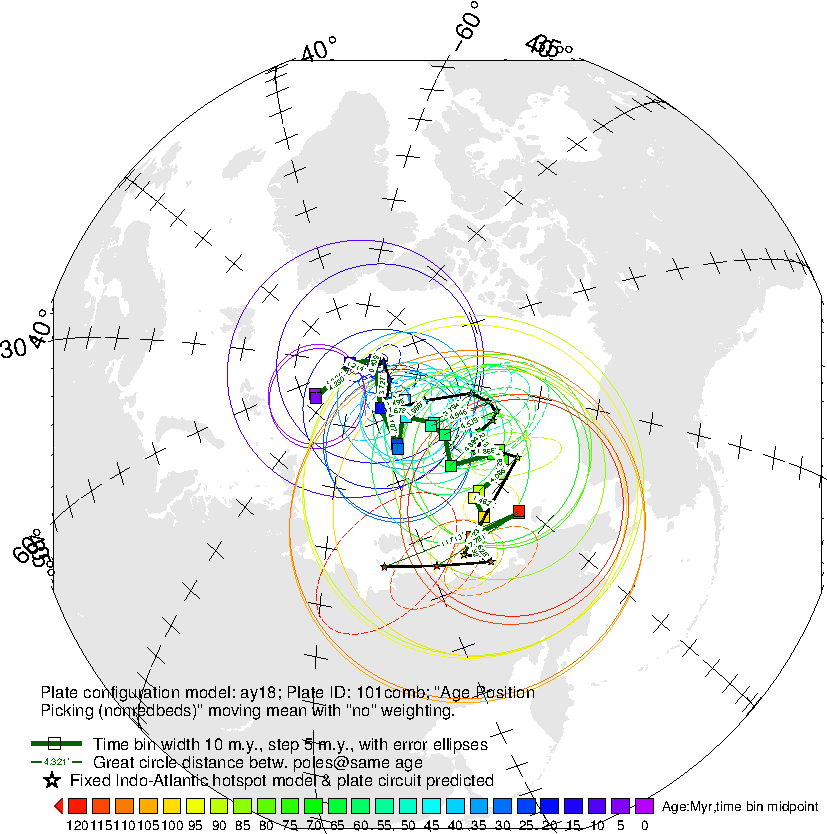
\includegraphics[width=\textwidth]{figures/ay18_101comb_10_5_11_0.pdf}
		\caption{North America (101): minimum 0.0053 (11, 0)}\label{fig-nac-105110} % subcaption
	\end{subfigure}
	\begin{subfigure}{.42\textwidth} % width of right subfigure
		\includegraphics[width=\textwidth]{figures/ay18_101comb_10_5_16_3.pdf}
		\caption{North America (101): maximum 0.0921 (16, 3)}\label{fig-nac-105163} % subcaption
	\end{subfigure}
	\vspace{.1em} % here you can insert horizontal or vertical space
	\begin{subfigure}{.42\textwidth}
		\includegraphics[width=\textwidth]{figures/ay18_501comb_10_5_19_0.pdf}
		\caption{India (501): minimum 0.023 (19, 0)}\label{fig-ind-105190}
	\end{subfigure}
	\begin{subfigure}{.42\textwidth}
		\includegraphics[width=\textwidth]{figures/ay18_501comb_10_5_8_3.pdf}
		\caption{India (501): maximum 0.5137 (8, 3)}\label{fig-ind-10583}
	\end{subfigure}
	\vspace{.1em}
	\begin{subfigure}{.42\textwidth}
		\includegraphics[width=\textwidth]{figures/ay18_801comb_10_5_17_0.pdf}
		\caption{Australia (801): minimum 0.0037 (17, 0)}\label{fig-au-105170}
	\end{subfigure}
	\begin{subfigure}{.42\textwidth}
		\includegraphics[width=\textwidth]{figures/ay18_801comb_10_5_22_3.pdf}
		\caption{Australia (801): maximum 0.3954 (22, 3)}\label{fig-au-105223}
	\end{subfigure}
	\caption[Best and worst differences with test (10 Myr bin, 5 Myr
step)]{Path comparisons with best and worst difference values shown in
Fig.~\ref{fig-dif}.}\label{fig-difbw}
\end{figure*}

\begin{figure*}
	\centering
	\begin{subfigure}{1.01\textwidth}
		\includegraphics[width=\textwidth]{figures/f501d101.pdf}
		\caption{India (501) - North America (101)}\label{fig-i-n-dif}
	\end{subfigure}
	\vspace{1em}
	\begin{subfigure}{1.01\textwidth}
		\includegraphics[width=\textwidth]{figures/f801d101.pdf}
		\caption{Australia (801) - North America (101)}\label{fig-a-n-dif}
	\end{subfigure}
	\vspace{1em}
	\begin{subfigure}{1.01\textwidth}
		\includegraphics[width=\textwidth]{figures/f501d801.pdf}
		\caption{India (501) - Australia (801)}\label{fig-i-a-dif}
	\end{subfigure}
	\caption[Differences of differences with test of each plate's paleomagnetic
APWPs versus its FHM predicted APWP]{Differences between grids in
Fig.~\ref{fig-dif}. The absolute difference values less than
1.96-standard-deviation interval of the whole 168 values are labeled in green,
more than 1.96-standard-deviation interval labeled in red.}\label{fig-d-dif}
\end{figure*}

\subparagraph{Measure 2: Only Space Tested}

According to the results (Fig.~\ref{fig-nant-dif}, Fig.~\ref{fig-indnt-dif} and
Fig.~\ref{fig-aunt-dif}), we can observe:
%
\begin{enumerate}
  \item the groups of picking-method-no 1, 19, 21 and 25 are the best, and 2
        and 14 the worst, for all the three continents.
\end{enumerate}

\begin{figure*}
	\centering
	\begin{subfigure}{1.01\textwidth} % width of left subfigure
		\includegraphics[width=\textwidth]{figures/101_120_0_.pdf}
		\caption{North America (101): minimum 0.2536 (1, 1), maximum 0.5104 (14, 4), mean 0.3837, median 0.3912}\label{fig-nant-dif} % subcaption
	\end{subfigure}
	\vspace{.1em} % here you can insert horizontal or vertical space
	\begin{subfigure}{1.01\textwidth} % width of right subfigure
		\includegraphics[width=\textwidth]{figures/501_120_0_.pdf}
		\caption{India (501): minimum 0.282 (6, 5), maximum 0.7637 (8, 3), mean 0.4667, median 0.4532}\label{fig-indnt-dif} % subcaption
	\end{subfigure}
	\vspace{.1em}
	\begin{subfigure}{1.01\textwidth}
		\includegraphics[width=\textwidth]{figures/801_120_0_.pdf}
		\caption{Australia (801): minimum 0.2246 (11, 0), maximum 0.7554 (22, 3), mean 0.502, median 0.5142}\label{fig-aunt-dif} % subcaption
	\end{subfigure}
	\caption[Differences without shape test of each plate's paleomagnetic APWPs
versus its FHM predicted APWP]{Difference values without shape test between each
continent's paleomagnetic APWPs and its predicted APWP from FHM and related
plate circuit. The paths are in 10 Myr bin and 5 Myr step. The difference values
less than one-standard-deviation interval of the whole 168 values are labeled in
green, more than one-standard-deviation interval labeled in
red.}\label{fig-difnt} % caption for whole figure
\end{figure*}

\begin{figure*}
	\centering
	\begin{subfigure}{.42\textwidth}
		\includegraphics[width=\textwidth]{figures/ay18_101comb_10_5_1_1.pdf}
		\caption{North America (101): minimum 0.2536 (1, 1)}\label{fig-nant-10511}
	\end{subfigure}
	\begin{subfigure}{.42\textwidth}
		\includegraphics[width=\textwidth]{figures/ay18_101comb_10_5_14_4.pdf}
		\caption{North America (101): maximum 0.5104 (14, 4)}\label{fig-nant-105144}
	\end{subfigure}
	\vspace{.1em}
	\begin{subfigure}{.42\textwidth}
		\includegraphics[width=\textwidth]{figures/ay18_501comb_10_5_6_5.pdf}
		\caption{India (501): minimum 0.282 (6, 5)}\label{fig-indnt-10565}
	\end{subfigure}
	\begin{subfigure}{.42\textwidth}
		\includegraphics[width=\textwidth]{figures/ay18_501comb_10_5_8_3.pdf}
		\caption{India (501): maximum 0.7637 (8, 3), same as Fig.~\ref{fig-ind-10583}}\label{fig-indnt-10583}
	\end{subfigure}
	\vspace{.1em}
	\begin{subfigure}{.42\textwidth}
		\includegraphics[width=\textwidth]{figures/ay18_801comb_10_5_11_0.pdf}
		\caption{Australia (801): minimum 0.2246 (11, 0)}\label{fig-aunt-105110}
	\end{subfigure}
	\begin{subfigure}{.42\textwidth}
		\includegraphics[width=\textwidth]{figures/ay18_801comb_10_5_22_3.pdf}
		\caption{Australia (801): maximum 0.7554 (22, 3), same as Fig.~\ref{fig-au-105223}}\label{fig-aunt-105223}
	\end{subfigure}
	\caption[Best and worst differences without shape test (10 Myr bin, 5 Myr
step)]{Path comparisons with best and worst difference values shown in
Fig.~\ref{fig-difnt}.}\label{fig-difntbw}
\end{figure*}

\paragraph{20 Myr Binning and 10 Myr Stepping}

\subparagraph{Measure 1: Both Space and Shape Tested}

According to the results (Fig.~\ref{fig-dif2010}), we can observe:
%
\begin{enumerate}
  \item the groups of picking-method-no 19 is the best, and 16 the worst, for
        all the three continents.
\end{enumerate}

\begin{figure*}
	\centering
	\begin{subfigure}{1.01\textwidth} % width of left subfigure
		\includegraphics[width=\textwidth]{figures/101_20_10_120_0.pdf}
		\caption{North America (101): minimum 0.0115 (13, 0), maximum 0.0635 (16, 2), mean 0.0335, median 0.0285}\label{fig-nac-dif2010} % subcaption
	\end{subfigure}
	\vspace{1em} % here you can insert horizontal or vertical space
	\begin{subfigure}{1.01\textwidth} % width of right subfigure
		\includegraphics[width=\textwidth]{figures/501_20_10_120_0.pdf}
		\caption{India (501): minimum 0.0143 (6, 3), maximum 0.1543 (16, 3), mean 0.074, median 0.0755}\label{fig-ind-dif2010} % subcaption
	\end{subfigure}
	\vspace{1em}
	\begin{subfigure}{1.01\textwidth}
		\includegraphics[width=\textwidth]{figures/801_20_10_120_0.pdf}
		\caption{Australia (801): minimum 0.0022 (11, 0), maximum 0.3265 (22, 3), mean 0.0686, median 0.0346}\label{fig-au-dif2010} % subcaption
	\end{subfigure}
	\caption[Differences with test of each plate's paleomagnetic APWPs versus
its FHM predicted APWP]{Same as Fig.~\ref{fig-dif}. The only difference is here
the paths are in 20 Myr bin and 10 Myr step. The difference values less than
one-standard-deviation interval of the whole 168 values are labeled in green,
more than one-standard-deviation interval labeled in red.}\label{fig-dif2010} % caption for whole figure
\end{figure*}

\begin{figure*}
	\centering
	\begin{subfigure}{.43\textwidth}
		\includegraphics[width=\textwidth]{figures/ay18_101comb_20_10_13_0.pdf}
		\caption{North America (101): minimum 0.0115 (13, 0)}\label{fig-nac-2010130}
	\end{subfigure}
	\begin{subfigure}{.43\textwidth}
		\includegraphics[width=\textwidth]{figures/ay18_101comb_20_10_16_2.pdf}
		\caption{North America (101): maximum 0.0635 (16, 2)}\label{fig-nac-2010162}
	\end{subfigure}
	\vspace{.1em}
	\begin{subfigure}{.43\textwidth}
		\includegraphics[width=\textwidth]{figures/ay18_501comb_20_10_6_3.pdf}
		\caption{India (501): minimum 0.0143 (6, 3)}\label{fig-ind-201063}
	\end{subfigure}
	\begin{subfigure}{.43\textwidth}
		\includegraphics[width=\textwidth]{figures/ay18_501comb_20_10_16_3.pdf}
		\caption{India (501): maximum 0.1543 (16, 3)}\label{fig-ind-2010163}
	\end{subfigure}
	\vspace{.1em}
	\begin{subfigure}{.43\textwidth}
		\includegraphics[width=\textwidth]{figures/ay18_801comb_20_10_11_0.pdf}
		\caption{Australia (801): minimum 0.0022 (11, 0)}\label{fig-au-2010110}
	\end{subfigure}
	\begin{subfigure}{.43\textwidth}
		\includegraphics[width=\textwidth]{figures/ay18_801comb_20_10_22_3.pdf}
		\caption{Australia (801): maximum 0.3265 (22, 3)}\label{fig-au-2010223}
	\end{subfigure}
	\caption[Best and worst differences with test (20 Myr bin, 10 Myr
step)]{Path comparisons with best and worst difference values shown in
Fig.~\ref{fig-dif2010}.}\label{fig-dif2010bw}
\end{figure*}

\subparagraph{Measure 2: Only Space Tested}

According to the results (Fig.~\ref{fig-dif2010nt}), we can observe:
%
\begin{enumerate}
  \item the groups of picking-method-no 11, 13, 19 and 21 are the best, and 16
        the worst, for all the three continents.
\end{enumerate}

\begin{figure*}
	\centering
	\begin{subfigure}{1.01\textwidth} % width of left subfigure
		\includegraphics[width=\textwidth]{figures/101_20_10_120_0_.pdf}
		\caption{North America (101): minimum 0.2768 (19, 0), maximum 0.4683 (14, 5), mean 0.3773, median 0.3855}\label{fig-nant-dif2010} % subcaption
	\end{subfigure}
	\vspace{.1em} % here you can insert horizontal or vertical space
	\begin{subfigure}{1.01\textwidth} % width of right subfigure
		\includegraphics[width=\textwidth]{figures/501_20_10_120_0_.pdf}
		\caption{India (501): minimum 0.2676 (7, 3), maximum 0.5027 (23, 1; 27, 1), mean 0.3914, median 0.408}\label{fig-indnt-dif2010} % subcaption
	\end{subfigure}
	\vspace{.1em}
	\begin{subfigure}{1.01\textwidth}
		\includegraphics[width=\textwidth]{figures/801_20_10_120_0_.pdf}
		\caption{Australia (801): minimum 0.1849 (11, 1), maximum 0.5772 (22, 2), mean 0.3882, median 0.3892}\label{fig-aunt-dif2010} % subcaption
	\end{subfigure}
	\caption[Differences without shape test of each plate's paleomagnetic APWPs
versus its FHM predicted APWP]{Same as Fig.~\ref{fig-difnt}. The only difference
is here the paths are in 20 Myr bin and 10 Myr step. The difference values less
than one-standard-deviation interval of the whole 168 values are labeled in
green, more than one-standard-deviation interval labeled in
red.}\label{fig-dif2010nt} % caption for whole figure
\end{figure*}

\begin{figure*}
	\centering
	\begin{subfigure}{.43\textwidth}
		\includegraphics[width=\textwidth]{figures/ay18_101comb_20_10_19_0.pdf}
		\caption{North America (101): minimum 0.2768 (19, 0)}\label{fig-nant-2010190}
	\end{subfigure}
	\begin{subfigure}{.43\textwidth}
		\includegraphics[width=\textwidth]{figures/ay18_101comb_20_10_14_5.pdf}
		\caption{North America (101): maximum 0.4683 (14, 5)}\label{fig-nant-2010145}
	\end{subfigure}
	\vspace{.1em}
	\begin{subfigure}{.43\textwidth}
		\includegraphics[width=\textwidth]{figures/ay18_501comb_20_10_7_3.pdf}
		\caption{India (501): minimum 0.2676 (7, 3)}\label{fig-indnt-201073}
	\end{subfigure}
	\begin{subfigure}{.43\textwidth}
		\includegraphics[width=\textwidth]{figures/ay18_501comb_20_10_23_1.pdf}
		\caption{India (501): maximum 0.5027 (23, 1; 27, 1)}\label{fig-indnt-2010231}
	\end{subfigure}
	\vspace{.1em}
	\begin{subfigure}{.43\textwidth}
		\includegraphics[width=\textwidth]{figures/ay18_801comb_20_10_11_1.pdf}
		\caption{Australia (801): minimum 0.1849 (11, 1)}\label{fig-aunt-2010111}
	\end{subfigure}
	\begin{subfigure}{.43\textwidth}
		\includegraphics[width=\textwidth]{figures/ay18_801comb_20_10_22_2.pdf}
		\caption{Australia (801): maximum 0.5772 (22, 2)}\label{fig-aunt-2010222}
	\end{subfigure}
	\caption[Best and worst differences without shape test (20 Myr bin, 10 Myr
step)]{Path comparisons with best and worst difference values shown in
Fig.~\ref{fig-dif2010nt}.}\label{fig-dif2010ntbw}
\end{figure*}

\subsubsection{When MHM and Plate Circuit Predicted APWP as Reference}

Then, we focus on analysing the results with MHM and plate circuit predicted
APWP (Fig.~\ref{fig-mhsPred}, Fig.~\ref{fig-mhsPred501},
Fig.~\ref{fig-mhsPred801}) as the reference path.

\begin{figure*}
	\centering
	\begin{subfigure}{1.01\textwidth} % width of left subfigure
		\includegraphics[width=\textwidth]{figures/101_120_0m.pdf}
		\caption{North America (101): minimum 0.00077 (4, 0), maximum 0.0926 (16, 5), mean 0.0361, median 0.0325}\label{fig-nac-difm} % subcaption
	\end{subfigure}
	\vspace{1em} % here you can insert horizontal or vertical space
	\begin{subfigure}{1.01\textwidth} % width of right subfigure
		\includegraphics[width=\textwidth]{figures/501_120_0m.pdf}
		\caption{India (501): minimum 0.0228 (4, 3), maximum 0.5188 (8, 3), mean 0.113, median 0.0746}\label{fig-ind-difm} % subcaption
	\end{subfigure}
	\vspace{1em}
	\begin{subfigure}{1.01\textwidth}
		\includegraphics[width=\textwidth]{figures/801_120_0m.pdf}
		\caption{Australia (801): minimum 0.0024 (17, 5), maximum 0.3662 (22, 3), mean 0.0744, median 0.0374}\label{fig-au-difm} % subcaption
	\end{subfigure}
	\caption[Differences with test of each plate's paleomagnetic APWPs versus
its MHM predicted APWP]{Same as Fig.~\ref{fig-dif} except that the reference
path is predicted from MHM here.}\label{fig-difm} % caption for whole figure
\end{figure*}

\begin{figure*}
	\centering
	\begin{subfigure}{.42\textwidth}
		\includegraphics[width=\textwidth]{figures/ay18_101comb_10_5_4_0m.pdf}
		\caption{North America (101): minimum 0.00077 (4, 0)}\label{fig-nac-10540m}
	\end{subfigure}
	\begin{subfigure}{.42\textwidth}
		\includegraphics[width=\textwidth]{figures/ay18_101comb_10_5_16_5m.pdf}
		\caption{North America (101): maximum 0.0926 (16, 5)}\label{fig-nac-105165m}
	\end{subfigure}
	\vspace{.1em}
	\begin{subfigure}{.42\textwidth}
		\includegraphics[width=\textwidth]{figures/ay18_501comb_10_5_4_3m.pdf}
		\caption{India (501): minimum 0.0228 (4, 3)}\label{fig-ind-10543m}
	\end{subfigure}
	\begin{subfigure}{.42\textwidth}
		\includegraphics[width=\textwidth]{figures/ay18_501comb_10_5_8_3m.pdf}
		\caption{India (501): maximum 0.5188 (8, 3)}\label{fig-ind-10583m}
	\end{subfigure}
	\vspace{.1em}
	\begin{subfigure}{.42\textwidth}
		\includegraphics[width=\textwidth]{figures/ay18_801comb_10_5_17_5m.pdf}
		\caption{Australia (801): minimum 0.0024 (17, 5)}\label{fig-au-105175m}
	\end{subfigure}
	\begin{subfigure}{.42\textwidth}
		\includegraphics[width=\textwidth]{figures/ay18_801comb_10_5_22_3m.pdf}
		\caption{Australia (801): maximum 0.3662 (22, 3)}\label{fig-au-105223m}
	\end{subfigure}
	\caption[Best and worst differences with test (10 Myr bin, 5 Myr
step)]{Path comparisons with best and worst difference values shown in
Fig.~\ref{fig-difm}.}\label{fig-difbwm}
\end{figure*}

\paragraph{10 Myr Binning and 5 Myr Stepping}

\subparagraph{Measure 1: Both Space and Shape Tested}

According to the results (Fig.~\ref{fig-nac-difm}, Fig.~\ref{fig-ind-difm} and
Fig.~\ref{fig-au-difm}), we can observe:
%
\begin{enumerate}
  \item there is no best picking method, whereas no. 16 is the worst, for all
		the three continents.
\end{enumerate}

\begin{figure*}
	\centering
	\begin{subfigure}{1.01\textwidth} % width of left subfigure
		\includegraphics[width=\textwidth]{figures/101_120_0_m.pdf}
		\caption{North America (101): minimum 0.2147 (11, 0), maximum 0.5183 (16, 3), mean 0.3702, median 0.3642}\label{fig-nant-difm} % subcaption
	\end{subfigure}
	\vspace{.1em} % here you can insert horizontal or vertical space
	\begin{subfigure}{1.01\textwidth} % width of right subfigure
		\includegraphics[width=\textwidth]{figures/501_120_0_m.pdf}
		\caption{India (501): minimum 0.2961 (26, 3), maximum 0.7779 (8, 3), mean 0.4578, median 0.4306}\label{fig-indnt-difm} % subcaption
	\end{subfigure}
	\vspace{.1em}
	\begin{subfigure}{1.01\textwidth}
		\includegraphics[width=\textwidth]{figures/801_120_0_m.pdf}
		\caption{Australia (801): minimum 0.2008 (11, 1), maximum 0.7136 (26, 4), mean 0.46, median 0.4726}\label{fig-aunt-difm} % subcaption
	\end{subfigure}
	\caption[Differences without shape test of each plate's paleomagnetic APWPs
versus its MHM predicted APWP]{Same as Fig.~\ref{fig-difnt} except that the
reference path is predicted from MHM here.}\label{fig-difntm} % caption for whole figure
\end{figure*}

\begin{figure*}
	\centering
	\begin{subfigure}{.42\textwidth}
		\includegraphics[width=\textwidth]{figures/ay18_101comb_10_5_11_0m.pdf}
		\caption{North America (101): minimum 0.2147 (11, 0)}\label{fig-nant-105110m}
	\end{subfigure}
	\begin{subfigure}{.42\textwidth}
		\includegraphics[width=\textwidth]{figures/ay18_101comb_10_5_16_3m.pdf}
		\caption{North America (101): maximum 0.5183 (16, 3)}\label{fig-nant-105163m}
	\end{subfigure}
	\vspace{.1em}
	\begin{subfigure}{.42\textwidth}
		\includegraphics[width=\textwidth]{figures/ay18_501comb_10_5_26_3m.pdf}
		\caption{India (501): minimum 0.2961 (26, 3)}\label{fig-indnt-105263m}
	\end{subfigure}
	\begin{subfigure}{.42\textwidth}
		\includegraphics[width=\textwidth]{figures/ay18_501comb_10_5_8_3m.pdf}
		\caption{India (501): maximum 0.7779 (8, 3), same as Fig.~\ref{fig-ind-10583m}}\label{fig-indnt-10583m}
	\end{subfigure}
	\vspace{.1em}
	\begin{subfigure}{.42\textwidth}
		\includegraphics[width=\textwidth]{figures/ay18_801comb_10_5_11_1m.pdf}
		\caption{Australia (801): minimum 0.2008 (11, 1)}\label{fig-aunt-105111m}
	\end{subfigure}
	\begin{subfigure}{.42\textwidth}
		\includegraphics[width=\textwidth]{figures/ay18_801comb_10_5_26_4m.pdf}
		\caption{Australia (801): maximum 0.7136 (26, 4)}\label{fig-aunt-105264m}
	\end{subfigure}
	\caption[Best and worst differences without shape test (10 Myr bin, 5 Myr
step)]{Path comparisons with best and worst difference values shown in
Fig.~\ref{fig-difntm}.}\label{fig-difntbwm}
\end{figure*}

\subparagraph{Measure 2: Only Space Tested}

According to the results (Fig.~\ref{fig-nant-difm}, Fig.~\ref{fig-indnt-difm}
and Fig.~\ref{fig-aunt-difm}), we can observe:
%
\begin{enumerate}
  \item the groups of picking-method-no 1, 19 and 21 are the best, and 8, 10
        and 14 the worst, for all the three continents.
\end{enumerate}

\begin{figure*}
	\centering
	\begin{subfigure}{1.01\textwidth} % width of left subfigure
		\includegraphics[width=\textwidth]{figures/101_20_10_120_0m.pdf}
		\caption{North America (101): minimum 0.0058 (15, 5), maximum 0.1041 (8, 4), mean 0.0437, median 0.0267}\label{fig-nac-dif2010m} % subcaption
	\end{subfigure}
	\vspace{1em} % here you can insert horizontal or vertical space
	\begin{subfigure}{1.01\textwidth} % width of right subfigure
		\includegraphics[width=\textwidth]{figures/501_20_10_120_0m.pdf}
		\caption{India (501): minimum 0.0177 (6, 3), maximum 0.162 (16, 3), mean 0.0759, median 0.0621}\label{fig-ind-dif2010m} % subcaption
	\end{subfigure}
	\vspace{1em}
	\begin{subfigure}{1.01\textwidth}
		\includegraphics[width=\textwidth]{figures/801_20_10_120_0m.pdf}
		\caption{Australia (801): minimum 0.0047 (23, 4), maximum 0.3158 (26, 3), mean 0.0638, median 0.0307}\label{fig-au-dif2010m}
	\end{subfigure}
	\caption[Differences with test of each plate's paleomagnetic APWPs versus
its MHM predicted APWP]{Same as Fig.~\ref{fig-dif2010} except that the reference
path is predicted from MHM here.}\label{fig-dif2010m} % caption for whole figure
\end{figure*}

\begin{figure*}
	\centering
	\begin{subfigure}{.43\textwidth}
		\includegraphics[width=\textwidth]{figures/ay18_101comb_20_10_15_5m.pdf}
		\caption{North America (101): minimum 0.0058 (15, 5)}\label{fig-nac-2010155m}
	\end{subfigure}
	\begin{subfigure}{.43\textwidth}
		\includegraphics[width=\textwidth]{figures/ay18_101comb_20_10_8_4m.pdf}
		\caption{North America (101): maximum 0.1041 (8, 4)}\label{fig-nac-201084m}
	\end{subfigure}
	\vspace{.1em}
	\begin{subfigure}{.43\textwidth}
		\includegraphics[width=\textwidth]{figures/ay18_501comb_20_10_6_3m.pdf}
		\caption{India (501): minimum 0.0177 (6, 3)}\label{fig-ind-201063m}
	\end{subfigure}
	\begin{subfigure}{.43\textwidth}
		\includegraphics[width=\textwidth]{figures/ay18_501comb_20_10_16_3m.pdf}
		\caption{India (501): maximum 0.162 (16, 3)}\label{fig-ind-2010163m}
	\end{subfigure}
	\vspace{.1em}
	\begin{subfigure}{.43\textwidth}
		\includegraphics[width=\textwidth]{figures/ay18_801comb_20_10_23_4m.pdf}
		\caption{Australia (801): minimum 0.0047 (23, 4)}\label{fig-au-2010234m}
	\end{subfigure}
	\begin{subfigure}{.43\textwidth}
		\includegraphics[width=\textwidth]{figures/ay18_801comb_20_10_26_3m.pdf}
		\caption{Australia (801): maximum 0.3158 (26, 3)}\label{fig-au-2010263m}
	\end{subfigure}
	\caption[Best and worst differences with test (20 Myr bin, 10 Myr
step)]{Path comparisons with best and worst difference values shown in
Fig.~\ref{fig-dif2010m}.}\label{fig-dif2010bwm}
\end{figure*}

\paragraph{20 Myr Binning and 10 Myr Stepping}

\subparagraph{Measure 1: Both Space and Shape Tested}

According to the results (Fig.~\ref{fig-dif2010m}), we can observe:
%
\begin{enumerate}
  \item there is no best picking method, whereas no. 16 is the worst, for all
		the three continents.
\end{enumerate}

\begin{figure*}
	\centering
	\begin{subfigure}{1.01\textwidth} % width of left subfigure
		\includegraphics[width=\textwidth]{figures/101_20_10_120_0_m.pdf}
		\caption{North America (101): minimum 0.1923 (4, 0), maximum 0.4794 (16, 2), mean 0.3384, median 0.3318}\label{fig-nant-dif2010m} % subcaption
	\end{subfigure}
	\vspace{.1em} % here you can insert horizontal or vertical space
	\begin{subfigure}{1.01\textwidth} % width of right subfigure
		\includegraphics[width=\textwidth]{figures/501_20_10_120_0_m.pdf}
		\caption{India (501): minimum 0.2462 (6, 0), maximum 0.5417 (8, 3), mean 0.3858, median 0.3659}\label{fig-indnt-dif2010m} % subcaption
	\end{subfigure}
	\vspace{.1em}
	\begin{subfigure}{1.01\textwidth}
		\includegraphics[width=\textwidth]{figures/801_20_10_120_0_m.pdf}
		\caption{Australia (801): minimum 0.2091 (5, 5), maximum 0.5777 (14, 0), mean 0.3694, median 0.3676}\label{fig-aunt-dif2010m}
	\end{subfigure}
	\caption[Differences without shape test of each plate's paleomagnetic APWPs
versus its MHM predicted APWP]{Same as Fig.~\ref{fig-dif2010nt} except that the
reference path is predicted from MHM here.}\label{fig-dif2010ntm} % caption for whole figure
\end{figure*}

\begin{figure*}
	\centering
	\begin{subfigure}{.43\textwidth}
		\includegraphics[width=\textwidth]{figures/ay18_101comb_20_10_4_0m.pdf}
		\caption{North America (101): minimum 0.1923 (4, 0)}\label{fig-nant-201040m}
	\end{subfigure}
	\begin{subfigure}{.43\textwidth}
		\includegraphics[width=\textwidth]{figures/ay18_101comb_20_10_16_2m.pdf}
		\caption{North America (101): maximum 0.4794 (16, 2)}\label{fig-nant-2010162m}
	\end{subfigure}
	\vspace{.1em}
	\begin{subfigure}{.43\textwidth}
		\includegraphics[width=\textwidth]{figures/ay18_501comb_20_10_6_0m.pdf}
		\caption{India (501): minimum 0.2462 (6, 0)}\label{fig-indnt-201060m}
	\end{subfigure}
	\begin{subfigure}{.43\textwidth}
		\includegraphics[width=\textwidth]{figures/ay18_501comb_20_10_8_3m.pdf}
		\caption{India (501): maximum 0.5417 (8, 3)}\label{fig-indnt-201083m}
	\end{subfigure}
	\vspace{.1em}
	\begin{subfigure}{.43\textwidth}
		\includegraphics[width=\textwidth]{figures/ay18_801comb_20_10_5_5m.pdf}
		\caption{Australia (801): minimum 0.2091 (5, 5)}\label{fig-aunt-201055m}
	\end{subfigure}
	\begin{subfigure}{.43\textwidth}
		\includegraphics[width=\textwidth]{figures/ay18_801comb_20_10_14_0m.pdf}
		\caption{Australia (801): maximum 0.5777 (14, 0)}\label{fig-aunt-2010140m}
	\end{subfigure}
	\caption[Best and worst differences without shape test (20 Myr bin, 10 Myr
step)]{Path comparisons with best and worst difference values shown in
Fig.~\ref{fig-dif2010ntm}.}\label{fig-dif2010ntbwm}
\end{figure*}

\subparagraph{Measure 2: Only Space Tested}

According to the results (Fig.~\ref{fig-dif2010ntm}), we can observe:
%
\begin{enumerate}
  \item the groups of picking-method-no 15 and 19 are the best, and 8 the worst,
		for all the three continents.
\end{enumerate}

\subsubsection{Summary of Results}

\begin{table*}
\centering
\caption{Performance statistics of all the picking and weighting methods.}
\label{tab-bw}
\resizebox{\textwidth}{!}{%
\begin{tabular}{l|l|l|l|l|l|l|l|l|l|l|l|l|l}
\multicolumn{2}{l|}{\multirow{2}{*}{Grid}} & \multicolumn{2}{l|}{Best No.} &
  \multicolumn{2}{l|}{Worst No.} & \multirow{2}{*}{\parbox{1.8cm}{Proportion of
  APP Better Than AMP}} & \multicolumn{6}{l|}{\multirow{2}{*}{\parbox{5cm}{For
  All 28 Picking Methods, Count of Occurrences of Each Weighting No. Being
  Best}}} & \multirow{2}{*}{\parbox{2.6cm}{Picking 14/15 (Studies After 1983)
  Better Than 16/17 (Older)}} \\ \\ \cline{3-6} \cline{8-13}
\multicolumn{2}{l|}{} & Picking & Weighting & Picking & Weighting &  & 0 & 1 &
  2 & 3 & 4 & 5 &  \\ \hline
\multirow{12}{*}{FHM}
& Fig.~\ref{fig-nac-dif} & \multirow{2}{*}{\parbox{2cm}{1, 4, 5, 7, 11, 13, 15,
  19, 21, 25}} & \multirow{2}{*}{\parbox{1cm}{0, 1, 5}} &
  \multirow{2}{*}{\parbox{2cm}{2, 5, 7, 8, 14, 16, 17, 18, 22, 26}} &
  \multirow{2}{*}{\parbox{1cm}{0, 1, 2, 3, 4, 5}} & 27/28 & 15 & 4 & 2 & 3 & 1
  & 4 & Y/Y \\ \\ \cline{2-14}
& Fig.~\ref{fig-nant-dif} & \multirow{2}{*}{\parbox{2cm}{1, 11, 13, 15, 19, 21, 25}} &
  \multirow{2}{*}{\parbox{1cm}{0, 1, 2, 4, 5}} &
  \multirow{2}{*}{\parbox{2.4cm}{0, 2, 3, 8, 10, 12, 14, 16, 17, 18, 20, 24}} &
  \multirow{2}{*}{\parbox{1cm}{0, 1, 2, 3, 4, 5}} & 71/84 & 9 & 13 & 0 & 1 & 1
  & 4 & N/Y \\ \\ \cline{2-14}
& Fig.~\ref{fig-ind-dif} & \multirow{2}{*}{\parbox{2cm}{4, 5, 6, 7, 9, 19, 21}} &
  \multirow{2}{*}{\parbox{1cm}{0, 1, 2, 3, 4, 5}} &
  \multirow{2}{*}{\parbox{2.4cm}{0, 2, 8, 10, 12, 16, 18, 20, 24}} &
  \multirow{2}{*}{\parbox{1cm}{0, 1, 2, 3, 4, 5}} & 11/14 & 17 & 1 & 2 & 7 & 1
  & 0 & Y/Y \\ \\ \cline{2-14}
& Fig.~\ref{fig-indnt-dif} & \multirow{2}{*}{\parbox{2cm}{1, 4, 6, 9, 17, 19, 21,
  25, 26}} & \multirow{2}{*}{\parbox{1cm}{0, 1, 2, 3, 4, 5}} &
  \multirow{2}{*}{\parbox{2.4cm}{0, 2, 8, 10, 12, 14, 16, 18, 24}} &
  \multirow{2}{*}{\parbox{1cm}{0, 1, 2, 3, 4, 5}} & 5/7 & 13 & 1 & 4 & 5 & 0 &
  5& Y(4y2n)/Y(4y2n) \\ \\ \cline{2-14}
& Fig.~\ref{fig-au-dif} & \multirow{2}{*}{\parbox{2cm}{1, 11, 13, 17, 19, 21, 25}} &
  \multirow{2}{*}{\parbox{1cm}{0, 1, 3, 5}} &
  \multirow{2}{*}{\parbox{2.4cm}{2, 6, 14, 16, 22, 26}} &
  \multirow{2}{*}{\parbox{1cm}{0, 1, 2, 3, 4, 5}} & 27/28 & 11 & 4 & 1 & 8 & 3
  & 1 & N/N \\ \\ \cline{2-14}
& Fig.~\ref{fig-aunt-dif} & \multirow{2}{*}{\parbox{2cm}{1, 7, 11, 13, 17, 19, 21, 25}} &
  \multirow{2}{*}{\parbox{1cm}{0, 1, 3, 5}} &
  \multirow{2}{*}{\parbox{2.4cm}{2, 6, 14, 22, 26}} &
  \multirow{2}{*}{\parbox{1cm}{0, 1, 2, 3, 4, 5}} & 1 & 9 & 6 & 2 & 7 & 2 & 2 &
  N/N \\ \\ \cline{2-14}
& Fig.~\ref{fig-nac-dif2010} & \multirow{2}{*}{\parbox{2cm}{1, 4, 5, 7, 11, 13,
  15, 19, 21, 25}} & \multirow{2}{*}{\parbox{1cm}{0, 1, 3, 5}} &
  \multirow{2}{*}{\parbox{2.4cm}{2, 6, 14, 22, 26}} &
  \multirow{2}{*}{\parbox{1cm}{0, 1, 2, 3, 4, 5}} & 3/4 & 18 & 6 & 0 & 2 & 4 &
  3 & N(5n1y)/Y \\ \\ \cline{2-14}
& Fig.~\ref{fig-nant-dif2010} & \multirow{2}{*}{\parbox{2cm}{1, 4, 5, 6, 7, 9,
  11, 13, 15, 19, 21, 25}} & \multirow{2}{*}{\parbox{1cm}{0, 1, 3, 5}} &
  \multirow{2}{*}{\parbox{2.4cm}{0, 3, 8, 10, 11, 12, 14, 16, 17, 18, 20, 24}}
  & \multirow{2}{*}{\parbox{1cm}{0, 1, 2, 3, 4, 5}} & 17/21 & 15 & 6 & 0 & 2 &
  3& 2 & N/Y \\ \\ \cline{2-14}
& Fig.~\ref{fig-ind-dif2010} & \multirow{2}{*}{\parbox{2cm}{4, 5, 6, 7, 19}} &
  \multirow{2}{*}{\parbox{1cm}{0, 1, 2, 3, 4, 5}} &
  \multirow{2}{*}{\parbox{2.4cm}{0, 2, 10, 12, 16, 18, 20, 23, 24, 27}} &
  \multirow{2}{*}{\parbox{1cm}{0, 1, 2, 3, 4, 5}} & 59/84 & 12 & 6 & 0 & 9 & 0
  & 1 & Y/Y(4y2n) \\ \\ \cline{2-14}
& Fig.~\ref{fig-indnt-dif2010} & \multirow{2}{*}{\parbox{2cm}{4, 5, 6, 7, 9, 11,
  13, 19, 21}} & \multirow{2}{*}{\parbox{1cm}{0, 1, 2, 3, 4, 5}} &
  \multirow{2}{*}{\parbox{2cm}{0, 2, 8, 10, 12, 16, 23, 24,
  27}} & \multirow{2}{*}{\parbox{1cm}{0, 1, 2, 3, 4, 5}} & 11/14 & 9 & 3 & 2 &
  8 & 3 & 3 & Y(4y2n)/N(5n1y) \\ \\ \cline{2-14}
& Fig.~\ref{fig-au-dif2010} & \multirow{2}{*}{\parbox{2cm}{1, 11, 13, 17, 19, 21,
  25}} & \multirow{2}{*}{\parbox{1cm}{0, 1, 3, 4, 5}} &
  \multirow{2}{*}{\parbox{2cm}{2, 14, 16, 22, 26}} &
  \multirow{2}{*}{\parbox{1cm}{0, 1, 2, 3, 4, 5}} & 41/42 & 7 & 9 & 0 & 11 & 1
  & 2 & N/N(4n2y) \\ \\ \cline{2-14}
& Fig.~\ref{fig-aunt-dif2010} & \multirow{2}{*}{\parbox{2cm}{1, 11, 13, 15, 17,
  19, 21, 25}} & \multirow{2}{*}{\parbox{1cm}{0, 1, 3, 5}} &
  \multirow{2}{*}{\parbox{2cm}{2, 4, 5, 14, 16, 22, 26}} &
  \multirow{2}{*}{\parbox{1cm}{0, 1, 2, 3, 4, 5}} & 41/42 & 6 & 8 & 0 & 10 & 1
  & 3 & N/N(4n2y) \\ \\ \hline
\multirow{12}{*}{MHM}
& Fig.~\ref{fig-nac-difm} & \multirow{2}{*}{\parbox{2cm}{1, 4, 5, 7, 11, 13, 15,
  21, 25}} & \multirow{2}{*}{\parbox{1cm}{0, 1, 2, 3, 4, 5}} &
  \multirow{2}{*}{\parbox{2.2cm}{0, 8, 10, 12, 14, 16, 17, 18, 20, 22, 24}} &
  \multirow{2}{*}{\parbox{1cm}{0, 1, 2, 3, 4, 5}} & 11/12 & 14 & 6 & 1 & 1 & 2
  & 4 & Y/Y \\ \\ \cline{2-14}
& Fig.~\ref{fig-nant-difm} & \multirow{2}{*}{\parbox{2cm}{1, 5, 7, 11, 13, 15,
  19, 21, 23, 25, 27}} &
  \multirow{2}{*}{\parbox{1cm}{0, 1, 3, 5}} &
  \multirow{2}{*}{\parbox{2.4cm}{0, 8, 10, 12, 14, 16, 17, 18, 24}} &
  \multirow{2}{*}{\parbox{1cm}{0, 1, 2, 3, 4, 5}} & 27/28 & 6 & 12 & 0 & 2 & 0
  & 8 & Y/Y \\ \\ \cline{2-14}
& Fig.~\ref{fig-ind-difm} & \multirow{2}{*}{\parbox{2cm}{4, 5, 6, 7, 19, 22, 26}} &
  \multirow{2}{*}{\parbox{1cm}{0, 1, 2, 3, 4, 5}} &
  \multirow{2}{*}{\parbox{2.4cm}{0, 2, 8, 10, 12, 16, 18, 20, 24}} &
  \multirow{2}{*}{\parbox{1cm}{0, 1, 2, 3, 4, 5}} & 11/14 & 12 & 3 & 0 & 9 & 1
  & 3 & Y/Y \\ \\ \cline{2-14}
& Fig.~\ref{fig-indnt-difm} & \multirow{2}{*}{\parbox{2cm}{1, 4, 6, 15, 17, 19, 21,
  22, 26}} & \multirow{2}{*}{\parbox{1cm}{0, 1, 2, 3, 4, 5}} &
  \multirow{2}{*}{\parbox{2.4cm}{0, 2, 8, 10, 12, 14, 16, 24}} &
  \multirow{2}{*}{\parbox{1cm}{0, 1, 2, 3, 4, 5}} & 61/84 & 0 & 1 & 7 & 6 & 3 &
  11 & Y/Y(4y2n) \\ \\ \cline{2-14}
& Fig.~\ref{fig-au-difm} & \multirow{2}{*}{\parbox{2cm}{1, 11, 13, 17, 19, 21, 25}} &
  \multirow{2}{*}{\parbox{1cm}{0, 1, 3, 5}} &
  \multirow{2}{*}{\parbox{2.4cm}{2, 14, 16, 22, 26}} &
  \multirow{2}{*}{\parbox{1cm}{0, 1, 2, 3, 4, 5}} & 20/21 & 8 & 5 & 1 & 9 & 4
  & 1 & N/N \\ \\ \cline{2-14}
& Fig.~\ref{fig-aunt-difm} & \multirow{2}{*}{\parbox{2cm}{1, 11, 13, 17, 19, 21, 25}} &
  \multirow{2}{*}{\parbox{1cm}{0, 1, 3, 5}} &
  \multirow{2}{*}{\parbox{2.4cm}{2, 6, 8, 10, 14, 18, 22, 26}} &
  \multirow{2}{*}{\parbox{1cm}{0, 1, 2, 3, 4, 5}} & 1 & 8 & 3 & 0 & 11 & 1 & 5 &
  N/N \\ \\ \cline{2-14}
& Fig.~\ref{fig-nac-dif2010m} & \multirow{2}{*}{\parbox{2cm}{4, 5, 7, 11,
  15, 22, 26}} & \multirow{2}{*}{\parbox{1cm}{0, 1, 2, 3, 4, 5}} &
  \multirow{2}{*}{\parbox{2.4cm}{0, 8, 10, 12, 14, 16, 18, 20, 24}} &
  \multirow{2}{*}{\parbox{1cm}{0, 1, 2, 3, 4, 5}} & 3/4 & 15 & 6 & 1 & 0 & 1 &
  5 & N(5n1y)/Y \\ \\ \cline{2-14}
& Fig.~\ref{fig-nant-dif2010m} & \multirow{2}{*}{\parbox{2cm}{1, 4, 5, 7,
  11, 13, 15, 19, 21, 25}} & \multirow{2}{*}{\parbox{1cm}{0, 1, 3, 4, 5}} &
  \multirow{2}{*}{\parbox{2.4cm}{0, 8, 10, 12, 14, 16, 18, 20, 24}} &
  \multirow{2}{*}{\parbox{1cm}{0, 1, 2, 3, 4, 5}} & 6/7 & 8 & 6 & 2 & 6 &
  3 & 3 & Y(5y1n)/Y(5y1n) \\ \\ \cline{2-14}
& Fig.~\ref{fig-ind-dif2010m} & \multirow{2}{*}{\parbox{2cm}{4, 5, 6, 7, 19}} &
  \multirow{2}{*}{\parbox{1cm}{0, 1, 2, 3, 4, 5}} &
  \multirow{2}{*}{\parbox{2.4cm}{0, 2, 10, 12, 16, 18, 23, 24, 27}} &
  \multirow{2}{*}{\parbox{1cm}{0, 1, 2, 3, 4, 5}} & 29/42 & 8 & 8 & 2 & 5 & 3
  & 2 & Y/N(5n1y) \\ \\ \cline{2-14}
& Fig.~\ref{fig-indnt-dif2010m} & \multirow{2}{*}{\parbox{2cm}{6, 9, 15,
  17, 19, 22, 23, 26, 27}} & \multirow{2}{*}{\parbox{1cm}{0, 1, 2, 3, 4, 5}} &
  \multirow{2}{*}{\parbox{2cm}{0, 2, 3, 8, 10, 12, 16, 18, 24}} &
  \multirow{2}{*}{\parbox{1cm}{1, 2, 3, 4, 5}} & 61/84 & 5 & 4 & 3 &
  5 & 3 & 8 & Y/N(5n1y) \\ \\ \cline{2-14}
& Fig.~\ref{fig-au-dif2010m} & \multirow{2}{*}{\parbox{2cm}{1, 11, 13, 15, 17, 19, 21,
  23, 25, 27}} & \multirow{2}{*}{\parbox{1cm}{0, 1, 2, 3, 4, 5}} &
  \multirow{2}{*}{\parbox{2cm}{2, 14, 16, 22, 26}} &
  \multirow{2}{*}{\parbox{1cm}{0, 1, 2, 3, 4, 5}} & 41/42 & 9 & 5 & 0 & 8 & 5
  & 1 & N/Y(4y2n) \\ \\ \cline{2-14}
& Fig.~\ref{fig-aunt-dif2010m} & \multirow{2}{*}{\parbox{2cm}{1, 5, 7, 11, 13, 15,
  19, 21, 23, 25}} & \multirow{2}{*}{\parbox{1cm}{0, 1, 3, 4, 5}} &
  \multirow{2}{*}{\parbox{2cm}{2, 6, 8, 14, 20, 22, 26}} &
  \multirow{2}{*}{\parbox{1cm}{0, 1, 2, 3, 4, 5}} & 1 & 7 & 4 & 0 & 12 & 4
  & 1 & N/Y(4y2n)
\end{tabular}%
}
\end{table*}

According to all the above results (Fig.~\ref{fig-dif}, Fig.~\ref{fig-difnt},
Fig.~\ref{fig-dif2010}, Fig.~\ref{fig-dif2010nt}), we can observe:
%
\begin{enumerate}
  \item the self-explanatory topography of bands indicates that the picking
        methods (Table.~\ref{tab-pick}) influence the similarity more than the
        weighting methods (Table.~\ref{tab-weit}) do.
  \item weighting is not always making similarities better. In fact, for quite
        many of the methods, no weighting is the best performer
		(Table.~\ref{tab-bw}).
  \item generally the APP methods (adding data to a time window with overlapping
        age selection criterion) produce better similarities than the AMP
        methods (Table.~\ref{tab-bw}).
  \item the picking method no 19 is always the best when the FHM predicted APWP
		is the reference.
  \item the weighting method no 0, 1 and 5 are generally producing better
        similarity than 2, 3 and 4.
  \item North America (101) owns better similarity results than Australia (801)
        and India (501), because its worst and mean composite differences are
		always less than the other two continents'.
  \item for both North America (101) and India (501), more recent studies
        generally give better results than (or results close to) older studies.
		However, this is not true for Australia (801) (Fig.~\ref{fig-au-dif} and
		Fig.~\ref{fig-aunt-dif}).
\end{enumerate}

\subsection{Discussions}

The following discussions will be in Q\&A style.

\subsubsection{Question: Why the APP methods generally produce better
similarities than AMP methods do?}

\begin{figure}
\centering
\includegraphics[width=.5\textwidth]{figures/a95gcd_10_5F.pdf}
\caption[APP spatially better than AMP]{Paleomagnetic APWPs' mean A95 versus
mean GCDs between Paleomagnetic APWP and FHM and plate circuit predicted APWP\@.
Starting points of the vectors are results from AMP, while ending points are
from APP.}\label{fig-A95GCD105F}
\end{figure}


\subsubsection{Question: Why the AMP methods sometimes unexceptionally produce
better similarities than APP methods do?}

\paragraph{Measure 1:}

For example, for Fig.~\ref{fig-nac-dif}, there are only three special (of 84 APP
vs. AMP comparisons) cases picking/weighting 4/3, 4/5, 6/3 better than 5/3, 5/5,
7/3 respectively. For the cases of 4/3 vs 5/3 and 6/3 vs 7/3, there are more
distinguishable $d_a$ and $d_l$ from the APP methods (Situation 1). For 4/5 vs
5/5, all $d_a$ and $d_l$ are indistinguishable, and the paleomagnetic APWP error
ellipses are generally much smaller from the APP methods than from the AMP
methods, whereas the coeval pole GCDs are generally not very different for APP
and AMP methods. This could further cause more distinguishable $d_s$ or greater
distinguishable mean $d_s$ from the APP methods (Situation 2). In addition, APP
potentially could generate more mean poles than AMP, because sometimes for some
sliding window there is no VGP at all for AMP\@. If so, because of small number
of VGPs, the newly produced mean poles by APP could be far from its contemporary
model-predicted pole. This also could potentially bring more distinguishable
$d_s$, $d_a$ and $d_l$ for APP\@. Admittedly, at the same time, the mean poles
at other ages also should be derived from more VGPs from APP, but the extended
mean poles from small number of VGPs should be extremely far from its
contemporary model-predicted pole, so when this negative effect is beyond the
positive effect the other mean poles contribute, the composite difference score
would increase (Situation 3). However this phenomenon seldom occur
(Table.~\ref{tab-bw}).

Situation 1: Fig.~\ref{fig-nac-dif2010} picking/weighting 22/3 vs 23/3.
Fig.~\ref{fig-nac-difm} 6/3 vs 7/3.

Situation 2: Fig.~\ref{fig-ind-dif} picking/weighting 4/0\textendash5 vs
5/0\textendash5, 22/3 vs 23/3, 26/3 vs 27/3; Fig.~\ref{fig-au-dif}
picking/weighting 4/2\textendash3 vs 5/2\textendash3, 4/5 vs 5/5.
Fig.~\ref{fig-nac-dif2010} picking/weighting 2/0\textendash5 vs
3/0\textendash5, 4/0\textendash2 vs 5/0\textendash2, 4/4 vs 5/4, 6/5 vs 7/5,
6/2\textendash3 vs 7/2\textendash3, 22/4\textendash5 vs 23/4\textendash5, 22/1
vs 23/1, 26/4 vs 27/4, 26/2 vs 27/2. Fig.~\ref{fig-ind-dif2010} 14/3 vs 15/3.
Fig.~\ref{fig-au-dif2010} 4/2 vs 5/2. Fig.~\ref{fig-nac-difm} 4/0\textendash1 vs
5/0\textendash1. Fig.~\ref{fig-ind-difm} 4/0\textendash4 vs 5/0\textendash4,
22/0\textendash1 vs 23/0\textendash1, 22/3\textendash4 vs 23/3\textendash4,
Fig.~\ref{fig-au-difm} 4/3 vs 5/3, 4/0 vs 5/0, 8/5 vs 9/5, 8/3 vs 9/3.
Fig.~\ref{fig-ind-dif2010m} 14/2\textendash3 vs 15/2\textendash3.
Fig.~\ref{fig-au-dif2010m} 4/4 vs 5/4.

Combination of both Situation 1 and Situation 2: Fig.~\ref{fig-ind-dif}
picking/weighting 22/0\textendash2 vs 23/0\textendash2, 22/4\textendash5 vs
23/4\textendash5, 26/0\textendash2 vs 27/0\textendash2, 26/4\textendash5 vs
27/4\textendash5, Fig.~\ref{fig-nac-dif2010} picking/weighting 26/0\textendash1
vs 27/0\textendash1. Fig.~\ref{fig-nac-difm} 4/3 vs 5/3. Fig.~\ref{fig-ind-difm}
22/2 vs 23/2, 22/5 vs 23/5, 26/0\textendash5 vs 27/0\textendash5.

Situation 3: Fig.~\ref{fig-ind-dif2010} picking/weighting 6/0\textendash5 vs
7/0\textendash5, 22/0\textendash5 vs 23/0\textendash5, 26/0\textendash5 vs
27/0\textendash5. Fig.~\ref{fig-nac-difm} 4/2\textendash5 vs 5/2\textendash5.
Fig.~\ref{fig-nac-dif2010m} 2/0\textendash5 vs 3/0\textendash5, 4/2 vs 5/2, 4/4
vs 5/4, 6/2 vs 7/2, 22/0\textendash5 vs 23/0\textendash5, 26/0\textendash5 vs
27/0\textendash5. Fig.~\ref{fig-ind-dif2010m} 6/0\textendash5 vs
7/0\textendash5, 22/0\textendash5 vs 23/0\textendash5, 26/0\textendash5 vs
27/0\textendash5.

\paragraph{Measure 2:}

For example, for Fig.~\ref{fig-nant-dif}, there are 13 special (of 84 APP vs.
AMP comparisons) cases. For the case of 2/3 vs 3/3, coeval segment angular
differences $d_a$ are greater from APP method than from AMP method (Situation
1). For the case of 2/0 vs 3/0, 4/5 vs 5/5, 16/2 vs 17/2, 22/0\textendash4 vs
23/0\textendash4, 26/0\textendash3 vs 27/0\textendash3, fraction of
distinguishable coeval poles are more from APP method than from AMP method
(Situation 2). In addition, segment angular differences $d_l$ could be greater
from APP method than from AMP method (Situation 3).

Situation 1: Fig.~\ref{fig-nant-dif2010} 10/4 vs 11/4.

Situation 2: Fig.~\ref{fig-indnt-dif} picking/weighting 4/0\textendash5 vs
5/0\textendash5, 6/0\textendash5 vs 7/0\textendash5, 22/0\textendash5 vs
23/0\textendash5, 26/0\textendash5 vs 27/0\textendash5.
Fig.~\ref{fig-nant-dif2010} 2/4\textendash5 vs 3/4\textendash5, 2/0\textendash2
vs 3/0\textendash2, 4/1\textendash2 vs 5/1\textendash2, 4/4 vs 5/4, 6/0 vs 7/0,
6/4\textendash5 vs 7/4\textendash5, 22/4 vs 23/4. 26/4 vs 27/4, 26/0 vs 27/0.
Fig.~\ref{fig-indnt-difm} 6/0\textendash1 vs 7/0\textendash1, 6/3\textendash4 vs
7/3\textendash4. Fig.~\ref{fig-nant-dif2010m} 22/1 vs 23/1, 22/3\textendash4 vs
23/3\textendash4, 26/0\textendash1 vs 27/0\textendash1, 26/3\textendash5 vs
27/3\textendash5.

Combination of Situation 1 and Situation 2: Fig.~\ref{fig-nant-dif2010} 16/4 vs
17/4. Fig.~\ref{fig-indnt-dif2010} 22/0\textendash5 vs 23/0\textendash5.
26/0\textendash3 vs 27/0\textendash3, 26/5 vs 27/5. Fig.~\ref{fig-aunt-dif2010}
4/2 vs 5/2, 6/2 vs 7/2. Fig.~\ref{fig-nant-difm} 2/1 vs 3/1, 16/1\textendash2 vs
17/1\textendash2. Fig.~\ref{fig-indnt-difm} 4/0\textendash5 vs 5/0\textendash5,
22/0\textendash5 vs 23/0\textendash5, 26/0\textendash5 vs 27/0\textendash5.
Fig.~\ref{fig-nant-dif2010m} 4/4 vs 5/4, 4/2 vs 5/2

Situation 3: Fig.~\ref{fig-indnt-dif2010} 6/2 vs 7/2.

Combination of Situation 2 and Situation 3: Fig.~\ref{fig-indnt-difm} 6/2 vs
7/2.

Combination of Situation 1 and Situation 3: Fig.~\ref{fig-nant-dif2010m} 4/3 vs
5/3, 4/0 vs 5/0

Combination of Situations 1, 2 and 3: Fig.~\ref{fig-indnt-dif2010m}
6/0\textendash3 vs 7/0\textendash3, 14/2 vs 15/2, 22/0\textendash5 vs
23/0\textendash5, 26/0\textendash5 vs 27/0\textendash5.

\subsubsection{Question: Why weighting is not affecting?}

For Fig.~\ref{fig-nac-dif} Picking No (Pk) 0, Weighting No (Wt) 1\textendash4
cause 80\textendash85 Ma coeval segments distinguishable ($d_a$ and $d_l$) and
Wt 2 and 4 cause one more pair of distinguishable mean poles ($d_s$) than other
weighting methods. However, compared with Wt 0, Wt 5 does affect and bring a
better similarity, because Wt 5 decreases the GCDs of the 20, 80 and especially
100 Ma distinguishable pole pairs (by more than 2 degrees).

For Fig.~\ref{fig-nac-dif} Pk 1, Wt 2\textendash5 cause at least 3 more pairs of
distinguishable mean poles ($d_s$) than other weighting methods. Wt 1 increases
the GCDs of all the distinguishable pole pairs (0, 5 and 120 Ma).

For Fig.~\ref{fig-nac-dif} Pk 2, Wt 1\textendash5 cause at least 1 more pair of
distinguishable mean poles ($d_s$) than Wt 0 (60 Ma). Wt 4 increases another
pair of distinguishable mean poles ($d_s$) (80 Ma).


\subsubsection{Question: Why best and worst methods are not consistent?}
\paragraph{Question: Why the picking method 21 is not among the best for
20 Myr binning and 10 Myr stepping with both space and shape tested?}

As shown in Fig.~\ref{fig-dif}, Fig.~\ref{fig-difnt} and
Fig.~\ref{fig-dif2010nt}, both the picking methods 19 and 21 are among the
best. However, the picking method 21 is not one of the best any more for 20 Myr
binning and 10 Myr stepping with both space and shape tested
(Fig.~\ref{fig-dif2010}). Further, in fact, in Fig.~\ref{fig-dif2010}, we can
see the picking method 21 is still one of the best for North America (101) and
Australia (801), but just not for India (501). However, even for India (501),
the difference values (ranging 0.0483\textendash0.0535) produced by the picking
method 21 are still closer to the left bound of the one-standard-deviation
interval 0.0359\textendash0.1072 and relatively farther from the mean 0.074,
which means the picking method 21 is still a relatively better one.

\paragraph{Question: Why the picking method 16 is not among the worst for
10 Myr binning and 5 Myr stepping with only space tested?}

As shown in Fig.~\ref{fig-dif}, Fig.~\ref{fig-dif2010} and
Fig.~\ref{fig-dif2010nt}, the picking method 16 is always one of the worst.
However, the picking method 16 is not among the worst any more for 10 Myr
binning and 5 Myr stepping with only space tested (Fig.~\ref{fig-difnt}).
Further, in fact, in Fig.~\ref{fig-difnt}, we can see the picking method 16 is
still one of the worst for North America (101) and India (501), but just not for
Australia (801). However, even for Australia (801), the difference values
(ranging 0.564\textendash0.6144) produced by the picking method 16 are still
closer to the right bound of the one-standard-deviation interval
0.3102\textendash0.6548 and relatively farther from the mean 0.502, which means
the picking method 16 is still a relatively worse one.

\subsubsection{Question: Why the 10/5 bin/step methods sometimes unexceptionally
produce better similarities than the 20/10 methods do?}

\subsubsection{Question: Do time window size and step affect the results?}

A balance needs to be made between having windows that are too wide and steps
that are too long which will smooth the data so much we miss actual details in
the APWP (e.g.\ those 20 Myr window 10 Myr step paleomagnetic paths in
Fig~\ref{fig-dif2010bw} and Fig~\ref{fig-dif2010ntbw}) and windows that are too
narrow and steps that are too short which introduces noise by having too few
poles in each window (e.g.\ those 10 Myr window 5 Myr step paleomagnetic paths in
Fig~\ref{fig-difbw} and Fig~\ref{fig-difntbw}). There is a dependence here on
data density: higher density allows smaller windows/steps (this is one of the
things we want to test with selective data removal mentioned in Chapter 4).
Fitting curves by moving averaging change with different time window lengths and
time increment lengths (i.e.\ steps) (e.g., the similarity of the pair in
Fig~\ref{fig-au-2010223} is improved a bit compared to Fig~\ref{fig-au-105223}).
A variety of ways of binning the data (here both 20 Myr window 10 Myr step and
10 Myr window 5 Myr step) are being tested to see which one produces the better
and more appropriately smoothed fit.

\paragraph{What to expect is}
the difference values for 20/10 window/step should be generally lower than those
for 10/5 window/step, which further could result in more best methods and less
worst methods.

\paragraph{The results}
are summarised in Table.~\ref{tab-2010vs105F}.

\begin{table*}
\centering
\caption{Consistency check on comparisons of 20/10 window/step and 10/5
  window/step. Notes: E: expected; UE: unexpected.}
\label{tab-2010vs105F}
\resizebox{\textwidth}{!}{%
\begin{tabular}{l|l|l|l|p{2cm}|l|p{2.4cm}|l|lllllll}
\multicolumn{2}{c|}{Comparisons} & \multicolumn{3}{c|}{Consistency of Best} & \multicolumn{3}{c|}{Consistency of Worst} & \multicolumn{7}{c}{If Difference Values for 20/10 Bin/Step Are Lower (Y/N)} \\ \hline
\multicolumn{1}{c|}{10/5} & \multicolumn{1}{c|}{20/10} &
  \multicolumn{1}{c|}{Y/N} & \multicolumn{1}{c|}{Special Case(s)} &
  \multicolumn{1}{c|}{Notes} & \multicolumn{1}{c|}{Y/N} &
  \multicolumn{1}{c|}{Special Case(s)} & \multicolumn{1}{c|}{Notes} & \multicolumn{1}{c|}{Mean} & \multicolumn{1}{c|}{Median} & \multicolumn{1}{c|}{Maximum} & \multicolumn{1}{c|}{Minimum} & \multicolumn{1}{c|}{All} & \multicolumn{1}{c|}{If No, Unexpected Case (s)} & \multicolumn{1}{c}{Notes} \\ \hline
\multicolumn{15}{c}{FHM} \\ \hline
Fig.~\ref{fig-nac-dif} & Fig.~\ref{fig-nac-dif2010} & Y &\textendash &
  \multirow{2}{*}{\parbox{2cm}{Same: Picking no. 1, 4, 5, 7, 11, 13, 15, 19, 21 and 25}} &
  N & \multirow{2}{*}{\parbox{2.4cm}{Picking no. 2, 5, 7, 22 and 26 for
  10/5 (E); 0, 10, 12, 20 and 24 for 20/10 (UE)}} &
  \multirow{2}{*}{\parbox{2cm}{Same: Picking no. 8, 14, 16 and 18}} &
  \multicolumn{1}{l|}{N} & \multicolumn{1}{l|}{Y} & \multicolumn{1}{l|}{Y} &
  \multicolumn{1}{l|}{N} & \multicolumn{1}{l|}{N} &
  \multicolumn{1}{l|}{\multirow{2}{*}{\parbox{3cm}{(0,1,8,10,11,12,18,19,20,21,
  24,25)(0-5) (3,4,14),(0-3,5) (5,7,13,15),(0-2,4,5) 9,(0,2,4,5) 23,(2,3) 27,(0-2); account for 29/42}}} &
  \\ \\ \\ \\ \\ \hline
Fig.~\ref{fig-nant-dif} & Fig.~\ref{fig-nant-dif2010} & Y &
  \multirow{2}{*}{\parbox{2.5cm}{5 more best: Picking no. 4, 5, 6, 7 and 9 only for 20/10 (E)}} &
  \multirow{2}{*}{\parbox{2cm}{Same: Picking no. 1, 11, 13, 15, 19, 21 and 25}} &
  \multirow{2}{*}{\parbox{1cm}{N (almost Y)}} & \multirow{2}{*}{\parbox{2cm}{Picking no. 2 for 10/5 (E); 11 for 20/10 (UE)}} &
  \multirow{2}{*}{\parbox{2cm}{Same: Picking no. 0, 3, 8, 10, 12, 14, 16, 17, 18, 20 and 24}} &
  \multicolumn{1}{l|}{N} & \multicolumn{1}{l|}{Y} & \multicolumn{1}{l|}{Y} &
  \multicolumn{1}{l|}{N} & \multicolumn{1}{l|}{N} &
  \multicolumn{1}{l|}{\multirow{2}{*}{\parbox{3cm}{0,(1,3) (1,21),(0-5)
  3,(1,2,5) 4,5 5,(0,1,4) 7,(0,2,5) (8,11,13,25),(0-2,4,5) (9,27),(4,5)
  (10,12,20,24),1 15,(0,1,5) 17,4 19,(1,2,4,5) 22,(0-3,5) 26,(2,3,5); account
  for 17/42}}} &
  \\ \\ \\ \\ \\ \\ \\ \\ \hline
Fig.~\ref{fig-ind-dif} & Fig.~\ref{fig-ind-dif2010} & Y &
  \multirow{2}{*}{\parbox{2.5cm}{2 more best: Picking no. 9 and 21 only for 10/5 (UE)}} &
  \multirow{2}{*}{\parbox{2cm}{Same: Picking no. 4, 5, 6, 7 and 19}} &
  \multirow{2}{*}{\parbox{1cm}{N (almost Y)}} &
  \multirow{2}{*}{\parbox{2.4cm}{Picking no. 8 for 10/5 (E); 23 and 27 for 20/10 (UE)}} &
  \multirow{2}{*}{\parbox{2cm}{Same: Picking no. 0, 2, 10, 12, 16, 18, 20 and 24}} &
  \multicolumn{1}{l|}{Y} & \multicolumn{1}{l|}{Y} & \multicolumn{1}{l|}{Y} &
  \multicolumn{1}{l|}{Y} & \multicolumn{1}{l|}{N} &
  \multicolumn{1}{l|}{\multirow{2}{*}{\parbox{3cm}{15,3 19,(0,1,3,5) 21,0
  (22,26),(0-5) 23,(1,3,4) 27,(1,3); account for 23/168}}} &  \\ \\ \\ \\ \hline
Fig.~\ref{fig-indnt-dif} & Fig.~\ref{fig-indnt-dif2010} &
  \multirow{2}{*}{\parbox{1cm}{N (partially Y)}} &
  \multirow{2}{*}{\parbox{2.5cm}{Picking no. 1, 17, 25 and 26 for 10/5 (UE);
  5, 7, 11 and 13 for 20/10 (E)}} & \multirow{2}{*}{\parbox{2cm}{Same:
  Picking no. 4, 6, 9, 19 and 21}} & \multirow{2}{*}{\parbox{1cm}{N (almost Y)}} &
  \multirow{2}{*}{\parbox{2.4cm}{Picking no. 14 and 18 for 10/5 (E); 23 and 27 for 20/10 (UE)}} &
  \multirow{2}{*}{\parbox{2cm}{Same: Picking no. 0, 2, 8, 10, 12, 16 and 24}} &
  \multicolumn{1}{l|}{Y} & \multicolumn{1}{l|}{Y} & \multicolumn{1}{l|}{Y} &
  \multicolumn{1}{l|}{Y} & \multicolumn{1}{l|}{N} &
  \multicolumn{1}{l|}{\multirow{2}{*}{\parbox{3cm}{4,5 6,(3-5) 15,3 22,(3,5)
  23,(0-3) 26,(2,3,5) 27,(0,2,3); account for 17/168}}} &  \\ \\ \\ \\ \hline
Fig.~\ref{fig-au-dif} & Fig.~\ref{fig-au-dif2010} & Y &\textendash &
  \multirow{2}{*}{\parbox{2cm}{Same: Picking no. 1, 11, 13, 17, 19, 21 and 25}} &
  Y & \multirow{2}{*}{\parbox{2.4cm}{1 more worst: Picking no. 6 only for 10/5 (E)}} &
  \multirow{2}{*}{\parbox{2cm}{Same: Picking no. 2, 14, 16, 22 and 26}} &
  \multicolumn{1}{l|}{Y} & \multicolumn{1}{l|}{Y} & \multicolumn{1}{l|}{Y} &
  \multicolumn{1}{l|}{Y} & \multicolumn{1}{l|}{N} &
  \multicolumn{1}{l|}{\multirow{2}{*}{\parbox{3cm}{0,(1,2,5) (1,4,18,25),(0,1,3,5)
  7,0 (8,10,20),(2,5) 9,1 11,3 (12,24),(1,2) 13,(0,1,3) (14,22,26),(0-2,4,5)
  (16,17),(0-5) 19,5 21,(0,1,5); account for 33/84}}} &  \\ \\ \\ \\ \\ \\ \\ \\ \hline
Fig.~\ref{fig-aunt-dif} & Fig.~\ref{fig-aunt-dif2010} & \multirow{2}{*}{\parbox{1cm}{N (almost Y)}} &
  \multirow{2}{*}{\parbox{2.5cm}{Picking no. 7 for 10/5 (UE); 15 for 20/10 (E)}} &
  \multirow{2}{*}{\parbox{2cm}{Same: Picking no. 1, 11, 13, 17, 19, 21 and 25}} &
  N & \multirow{2}{*}{\parbox{2.4cm}{Picking no. 6 for 10/5 (E); 4, 5 and 16 for 20/10 (UE)}} &
  \multirow{2}{*}{\parbox{2cm}{Same: Picking no. 2, 14, 22 and 26}} &
  \multicolumn{1}{l|}{Y} & \multicolumn{1}{l|}{Y} & \multicolumn{1}{l|}{Y} &
  \multicolumn{1}{l|}{Y} & \multicolumn{1}{l|}{N} &
  \multicolumn{1}{l|}{\multirow{2}{*}{\parbox{3cm}{(1,25),(3,5) 5,2 13,3 17,5
  19,5 21,5; account for 9/168}}} &  \\ \\ \\ \hline
\multicolumn{15}{c}{MHM} \\ \hline
Fig.~\ref{fig-nac-difm} & Fig.~\ref{fig-nac-dif2010m} & N &
  \multirow{2}{*}{\parbox{2.5cm}{Picking no. 1, 13, 21 and 25 for 10/5 (UE);
  22 and 26 for 20/10 (E)}} &
  \multirow{2}{*}{\parbox{2cm}{Same: Picking no. 4, 5, 7, 11, and 15}} & Y &
  \multirow{2}{*}{\parbox{2.4cm}{2 more worst: Picking no. 17, 22 only for 10/5 (E)}} &
  \multirow{2}{*}{\parbox{2cm}{Same: Picking no. 0, 8, 10, 12, 14, 16, 18, 20 and 24}} &
  \multicolumn{1}{l|}{N} & \multicolumn{1}{l|}{Y} & \multicolumn{1}{l|}{N} &
  \multicolumn{1}{l|}{N} & \multicolumn{1}{l|}{N} &
  \multicolumn{1}{l|}{\multirow{2}{*}{\parbox{3cm}{(0,4,8,10,11,12,14,15,18, 20,24,25),(0-5)
  (1,19,21),(0,1,5) 3,5 (5,7),(0-2,4,5) 6,1 (9,13),(0,1,3,5) 23,(1,3)
  27,(1,3,5); account for 53/84}}} &
  \\ \\ \\ \\ \\ \\ \\ \hline
Fig.~\ref{fig-nant-difm} & Fig.~\ref{fig-nant-dif2010m} &
  \multirow{2}{*}{\parbox{1cm}{N (almost Y)}} &
  \multirow{2}{*}{\parbox{2.5cm}{Picking no. 23 and 27 for 10/5 (UE); 4 for 20/10 (E)}} &
  \multirow{2}{*}{\parbox{2cm}{Same: Picking no. 1, 5, 7, 11, 13, 15, 19, 21 and 25}} &
  \multirow{2}{*}{\parbox{1cm}{N (almost Y)}} &
  \multirow{2}{*}{\parbox{2cm}{Picking no. 17 for 10/5 (E); 20 for 20/10 (UE)}} &
  \multirow{2}{*}{\parbox{2cm}{Same: Picking no. 0, 8, 10, 12, 14, 16, 18 and 24}} &
  \multicolumn{1}{l|}{Y} & \multicolumn{1}{l|}{Y} & \multicolumn{1}{l|}{Y} &
  \multicolumn{1}{l|}{Y} & \multicolumn{1}{l|}{N} &
  \multicolumn{1}{l|}{\multirow{2}{*}{\parbox{3cm}{(0,3,21),5 (2,8,14),1
  9,(1,3,5) 10,(2,4) 11,(0,1,5) 15,(2-5) 20,2 23,(1,3) 25,4 27,(0,1,3,5);
  account for 13/84}}} &
  \\ \\ \\ \\ \\ \hline
Fig.~\ref{fig-ind-difm} & Fig.~\ref{fig-ind-dif2010m} & Y &
  \multirow{2}{*}{\parbox{2.5cm}{2 more best: Picking no. 22 and 26 only for 10/5 (UE)}} &
  \multirow{2}{*}{\parbox{2cm}{Same: Picking no. 4, 5, 6, 7 and 19}} &
  N & \multirow{2}{*}{\parbox{2.4cm}{Picking no. 8, 20 for 10/5 (E); 23 and 27 for 20/10 (UE)}} &
  \multirow{2}{*}{\parbox{2cm}{Same: Picking no. 0, 2, 10, 12, 16, 18 and 24}} &
  \multicolumn{1}{l|}{Y} & \multicolumn{1}{l|}{Y} & \multicolumn{1}{l|}{Y} &
  \multicolumn{1}{l|}{Y} & \multicolumn{1}{l|}{N} &
  \multicolumn{1}{l|}{\multirow{2}{*}{\parbox{3cm}{1,5 (4,15),3 (19,23,27),(0-5)
  21,(0,1,35) 22,(1,4) 25,(3,5) 26,4; account for 5/28}}} &  \\ \\ \\ \\ \hline
Fig.~\ref{fig-indnt-difm} & Fig.~\ref{fig-indnt-dif2010m} &
  \multirow{2}{*}{\parbox{1cm}{N (partially Y)}} &
  \multirow{2}{*}{\parbox{2.5cm}{Picking no. 1, 4 and 21 for 10/5 (UE);
  9, 23 and 27 for 20/10 (E)}} & \multirow{2}{*}{\parbox{2cm}{Same:
  Picking no. 6, 15, 17, 19, 22 and 26}} & \multirow{2}{*}{\parbox{1cm}{N (almost Y)}} &
  \multirow{2}{*}{\parbox{2.4cm}{Picking no. 14 for 10/5 (E); 3 and 18 for 20/10 (UE)}} &
  \multirow{2}{*}{\parbox{2cm}{Same: Picking no. 0, 2, 8, 10, 12, 16 and 24}} &
  \multicolumn{1}{l|}{Y} & \multicolumn{1}{l|}{Y} & \multicolumn{1}{l|}{Y} &
  \multicolumn{1}{l|}{Y} & \multicolumn{1}{l|}{N} &
  \multicolumn{1}{l|}{\multirow{2}{*}{\parbox{3cm}{4,5 15,(1-3) 19,2
  21,(4,5); account for 7/168}}} &  \\ \\ \\ \\ \hline
Fig.~\ref{fig-au-difm} & Fig.~\ref{fig-au-dif2010m} & Y &
  \multirow{2}{*}{\parbox{2.5cm}{3 more best: Picking no. 15, 23 and 27 only for 20/10 (E)}} &
  \multirow{2}{*}{\parbox{2cm}{Same: Picking no. 1, 11, 13, 17, 19, 21 and 25}} &
  Y &\textendash &
  \multirow{2}{*}{\parbox{2cm}{Same: Picking no. 2, 14, 16, 22 and 26}} &
  \multicolumn{1}{l|}{Y} & \multicolumn{1}{l|}{Y} & \multicolumn{1}{l|}{Y} &
  \multicolumn{1}{l|}{N} & \multicolumn{1}{l|}{N} &
  \multicolumn{1}{l|}{\multirow{2}{*}{\parbox{3cm}{(0,24),(1,2,5)
  (1,11,13,18,19,21,25),(0,1,3,5) 4,(0,3,5) (5,7),3 (8,17),(0-3,5) 12,(1-3,5)
  20,(1,2,4,5) 10,(1,2) (14,22,26),(0-2,4,5) 16,(0-5); account for 10/21}}} &  \\ \\ \\ \\ \\ \\ \\ \hline
Fig.~\ref{fig-aunt-difm} & Fig.~\ref{fig-aunt-dif2010m} &
  \multirow{2}{*}{\parbox{1cm}{N (almost Y)}} &
  \multirow{2}{*}{\parbox{2.5cm}{Picking no. 17 for 10/5 (UE); 5, 7, 15, 23 for 20/10 (E)}} &
  \multirow{2}{*}{\parbox{2cm}{Same: Picking no. 1, 11, 13, 19, 21 and 25}} &
  N & \multirow{2}{*}{\parbox{2.4cm}{Picking no. 10, 18 for 10/5 (E); 20 for 20/10 (UE)}} &
  \multirow{2}{*}{\parbox{2cm}{Same: Picking no. 2, 6, 8, 14, 22 and 26}} &
  \multicolumn{1}{l|}{Y} & \multicolumn{1}{l|}{Y} & \multicolumn{1}{l|}{Y} &
  \multicolumn{1}{l|}{N} & \multicolumn{1}{l|}{N} &
  \multicolumn{1}{l|}{\multirow{2}{*}{\parbox{3cm}{(1,11,19,21,25),(0,1,3,5)
  13,(0,1) 17,(0-3,5); account for 9/56}}} & 
\end{tabular}%
}
\end{table*}

\paragraph{Conclusions:}

\subparagraph{The APP methods (except with weighting no. 3) is recommended.}

\subparagraph{The different values for 20/10 window/step are indeed generally
lower than those for 10/5 window/step, excluding the unexpected case of North
America with both space and shape tested (Fig.~\ref{fig-nac-dif} and
Fig.~\ref{fig-nac-dif2010}).}


\section{Final Conclusions}

\begin{description}
  \item Picking method no. 16 (AMP with data from old studies) is not
		recommended, e.g.\ before 1983) for generating a paleomagnetic APWP.
\end{description}


\begin{acknowledgments}
All images are produced using GMT~\cite{W13}. Thanks to Ohio Supercomputer
Center for their remote HPC resources.
\end{acknowledgments}

\begin{thebibliography}{}
\bibitem[\protect\citename{Besse \& Courtillot }2002]{B02}
  Besse, J. \& Courtillot, V., 2002, Apparent and true polar wander and the
  geometry of the geomagnetic field over the last 200 Myr, \jgr{}\textbf{107},
  2300.
\bibitem[\protect\citename{Fisher }1953]{F53}
  Fisher, R. A., 1953. Dispersion on a sphere, \textit{Proc. Roy. Soc. London
  Ser. A.}, \textbf{217}, 295\textendash305.
\bibitem[\protect\citename{Jacox \& Samet }2007]{J07}
  Jacox, E. H. \& Samet, H., 2007. Spatial Join Techniques, \textit{ACM Trans.
  Database Syst.}. \textbf{32}, 7.
\bibitem[\protect\citename{King }1955]{K55}
  King, R. F., 1955. The remanent magnetism of artificially deposited sediments,
  \textit{Geophys. Suppl. Mon. Not. Roy. Astron. Soc. Lett.}, \textbf{7},
  115\textendash134.
\bibitem[\protect\citename{M{\"{u}}ller et al. }1993]{M93}
  M{\"{u}}ller, R. D., Royer, J. Y. \& Lawver, L. A., 1993. Revised plate
  motions relative to the hotspots from combined Atlantic and Indian-Ocean
  hotspot tracks, \textit{Geology}, \textbf{21}, 275\textendash278.
\bibitem[\protect\citename{M{\"{u}}ller et al. }1999]{M99}
  M{\"{u}}ller, R. D., Royer, J. Y., Cande, S. C., Roest, W. R. \& Maschenkov,
  S., 1999. New constraints on the Late Cretaceous/Tertiary plate tectonic
  evolution of the Caribbean, \textit{Sedimentary Basins of the World}.
  \textbf{4}, 33\textendash59.
\bibitem[\protect\citename{McQuarrie \& Wernicke }2006]{Mc06}
  McQuarrie, N. \& Wernicke, B. P., 2006. An animated tectonic reconstruction of
  southwestern North America since 36 Ma, \textit{Geosphere}, \textbf{1},
  147\textendash172.
\bibitem[\protect\citename{O'Neill et al. }2005]{O05}
  O'Neill, C., M{\"{u}}ller, R. D. \& Steinberger, B., 2005. On the
  uncertainties in hot spot reconstructions and the significance of moving hot
  spot reference frames, \textit{Geochem. Geophys. Geosyst.}, \textbf{6},
  Q04003.
\bibitem[\protect\citename{Pisarevsky }2005]{P05}
  Pisarevsky, S. A., 2005. New edition of the Global Paleomagnetic Database,
  \eos{}\textbf{86}, 170.
\bibitem[\protect\citename{Schettino \& Scotese }2005]{S05}
  Schettino, A. \& Scotese, C. R., 2005. Apparent polar wander paths for the
  major continents (200 Ma to the present day): a palaeomagnetic reference frame
  for global plate tectonic reconstructions, \gji{}\textbf{163},
  727\textendash759.
\bibitem[\protect\citename{Torsvik et al. }1992]{T92}
  Torsvik, T. H., Smethurst, M. A., van der Voo, R., Trench, A., Abrahamsen, N.
  \& Halvorsen, E., 1992. Baltica. A synopsis of Vendian-Permian palaeomagnetic
  data and their palaeotectonic implications, \textit{Earth Sci. Rev.},
  \textbf{33}, 133\textendash152.
\bibitem[\protect\citename{Torsvik \& Smethurst }1999]{T99}
  Torsvik, T. H. \& Smethurst, M. A., 1999. Plate tectonic modelling: virtual
  reality with GMAP, \textit{Comput. Geosci.}, \textbf{25}, 395\textendash402.
\bibitem[\protect\citename{Tauxe \& Kent }2004]{T04}
  Tauxe, L. \& Kent, D. V., 2004. A simplified statistical model for the
  geomagnetic field and the detection of shallow bias in paleomagnetic
  inclinations: Was the ancient magnetic field dipolar? \textit{Geophys.
  Monogr. AGU}, \textbf{145}, 101\textendash115.
\bibitem[\protect\citename{Torsvik et al. }2008]{T08}
  Torsvik, T. H., M{\"{u}}ller, R. D., van der Voo, R., Steinberger, B., \&
  Gaina, C., 2008. Global plate motion frames: Toward a unified model,
  \textit{Rev. Geophys.}, \textbf{46}, RG3004.
\bibitem[\protect\citename{Torsvik et al. }2012]{T12}
  Torsvik, T. H., van der Voo, R., Preeden, U., Mac Niocaill, C., Steinberger,
  B., Doubrovine, P. V., van Hinsbergen, D. J. J., Domeier, M., Gaina, C.,
  Tohver, E., Meert, J. G., McCausland, P. J. A. \& Cocks, L. R. M., 2012.
  Phanerozoic polar wander, palaeogeography and dynamics, \textit{Earth Sci.
  Rev.}, \textbf{114}, 325\textendash368.
\bibitem[\protect\citename{Tauxe et al. }2018]{T18}
  Tauxe L., Banerjee S.K., Butler R.F. \& van der Voo R., 2018.
  \textit{Essentials of Paleomagnetism}, 5th web edn, Available on line
\bibitem[\protect\citename{van der Voo }1990]{v90}
  van der Voo, R., 1990. The reliability of paleomagnetic data,
  \tecto{}\textbf{184}, 1\textendash9.
\bibitem[\protect\citename{Wessel et al. }2013]{W13}
  Wessel, P., Smith, W. H. F., Scharroo, R., Luis, J. \& Wobbe, F.,2013. Generic
  Mapping Tools: Improved version released, \eos{}\textbf{94}, 409\textendash410.
\bibitem[\protect\citename{Young et al. }2018]{Y18}
  Young, A., Flament, N., Maloney, K., Williams, S., Matthews, K., Zahirovic, S.
  \& Müller, D., 2018. Global kinematics of tectonic plates and subduction zones
  since the late Paleozoic Era, \textit{Geosci. Front.},
  \textbf{in press}, 000\textendash000.
\end{thebibliography}~\label{lastpage}
